\chapter{Successioni e Serie di Funzioni}
In questo capitolo verranno trattate Successioni e Serie di Funzioni di una sola variabile (in $\R$ o $\C$) a valori in $\R$ o $\C$. Molti dei risultati esposti (in particolare quelli di \fullref{sect:conv_punt}, \fullref{sect:conv_unif} e \fullref{sect:conv_quadr}) valgono anche in ambiti più generali.

La \fullref{sect:ser_funz_particol} invece non può essere facilmente estesa al caso di funzioni di più variabili, si veda \fullref{ex:conv_ser_piu_var}.

\vspace*{\baselineskip}
Questo capitolo si allontana dal corrispettivo nella dispensa ufficiale del corso al fine di fornire una spiegazione più discorsiva dell'argomento. Non è stato tralasciata alcuna delle definizioni, proposizioni o esercizi presenti nella dispensa, ma è stato aggiunto materiale.

Grazie alla dispensa di Sergio Rolando per la spiegazione chiara e dettagliata a cui si ispira la presente trattazione
\begin{center}
	\url{http://calvino.polito.it/~rolando/An2s_04_Successioni.Funzioni.pdf}
\end{center}

\section{Preliminari}\label{sect:prelim_serie_succ_funz}
Innanzitutto si ricorda la \fullref{def:succ}, cioè, dato un insieme $X \neq \emptyset$, una \textbf{Successione} è una funzione $x: \N \to X$ che associa ad ogni valore di $\N$ un elemento di $X$.

Si consideri ora la successione $x_n = x^n$, i cui termini sono
\[1 \qquad x^1 \qquad x^2  \qquad \dots \qquad x^n\]
Si tratta della \textbf{Successione Geometrica} di \textit{termine iniziale} $1$ e \textit{ragione} (la base) $x$. Questa successione può essere studiata con le conoscenze ottenute in \fullref{sect:succ_compl} fissando $x$ e facendo tendere $n$ ad $+\infty$.
\begin{example}
	\label{ex:conv_succ_xn}
	Studiare la convergenza della successione $x^n$, cioè il $\lim\limits_{n \to +\infty} x^n$
	\begin{solution}
		Fissando $x \in \R$ a diversi valori, studiando la successione numerica $x^n$ per $n \to \infty$ si ottiene
		\[
			\lim\limits_{n \to +\infty} x^n =
			\begin{cases}
				\begin{array}{ll}
					\nexists & \text{se } x \leq -1\\
					0 & \text{se } x \in \intervalopen{-1}{1}\\
					1 & \text{se } x = 1\\
					+\infty & \text{se } x > 1
				\end{array}
			\end{cases}
		\]
	\end{solution}
\end{example}

Cambiando però, dal punto di vista concettuale, i ruoli di $x$ ed $n$, cioè fissando $n$ e considerando $x$ come una variabile reale, si vede che ogni termine della successione è una \textbf{funzione} e che quindi la successione è \textbf{Successione di Funzioni}
\[f_0(x) = 1 \qquad f_1(x) = x^1 \qquad f_2(x) = x^2  \qquad \dots \qquad f_n(x) = x^n\]
\vspace*{-\baselineskip}
\begin{note}
	Le funzioni della successione, a rigore, si chiamano $f_0, f_1, f_2 ,\:\dotsc\:, f_n$ mentre i vari $f_\alpha(x) = x^\alpha$ sono i valori assunti da esse nel punto $x$
\end{note}
Si giunge dunque alla seguente definizione, tutt'altro che formale
\begin{definition}[Successione di Funzioni]
	\label{def:succ_funz}
	Si definisce \textbf{Successione di Funzioni} l'insieme
	\[\brackets{f_n:\; n \in \N} \text{ di funzioni } f_n:\; A \to \R\]
	dipendenti da un indice naturale $n$ (oltre cheda una variabile reale $x$) e definite su un \textbf{dominio comune} $A$.
\end{definition}

\begin{definition}[Successione delle Somme Parziali]
	\label{def:succ_somm_parz}
	Sia $X$ uno \textbf{Spazio Vettoriale} su $\R$ o su $\C$. Data una \textbf{Successione} $\brackets{x_n:\; n \in \N}$ di elementi di $X$, per ogni indice $k$ della successione si definisce una \textbf{Successione delle Somme Parziali}. Cioè il $k$\textit{-esimo} termine di $s$ è la somma dei termini da $0$ a $k$ della successione $x_n$:
	\[s_k = \sum\limits_{n = 0}^{k} x_n\]
	Quindi
	\begin{align*}
		s_0 &= x_0\\
		s_1 &= x_0 + x_1\\
		&\;\;\vdots\\
		s_k &= x_0 + x_1 + \dots + x_k
	\end{align*}
\end{definition}

\begin{definition}[Serie]
	\label{def:serie}
	Sia $X$ uno \textbf{Spazio Vettoriale} su $\R$ o su $\C$. Data una \textbf{Successione} $\brackets{x_n:\; n \in \N}$ di elementi di $X$, si definisce \textbf{Serie associata alla Successione} $x_n$ la somma di tutti i termini della successione:
	\[s = \sum\limits_{n = 0}^{+\infty} x_n = x_0 + x_1 + \dots\]
	Quindi si può definire la Serie usando la \fullref{def:succ_somm_parz} con $k \to +\infty$
	\[s = \lim\limits_{k \to +\infty} \sum\limits_{n = 0}^{k} x_n = \sum\limits_{n = 0}^{+\infty} x_n\]
\end{definition}
\begin{observation}
	Le \fullref{def:succ_somm_parz} e \fullref{def:serie} non fanno esplicitamente riferimento a successioni del tipo di \fullref{def:succ_funz}, ma ovviamente valgono anche quando $x_n$ è Successione di Funzioni.
\end{observation}
\begin{observation}
	La \fullref{def:serie} è intimamente legata alla \fullref{def:succ_somm_parz}, infatti per studiare il comportamento della Serie basta studiare la Successione delle Somme Parziali per $k \to +\infty$. Di conseguenza:
	\begin{align*}
		\text{La Serie è \textbf{Limitata}} \quad &\bydef \quad \text{La Successione delle Somme Parziali è \textbf{Limitata}}\\
		\text{La Serie è \textbf{Illimitata}} \quad &\bydef \quad \text{La Successione delle Somme Parziali è \textbf{Illimitata}}\\
		\text{La Serie è \textbf{Convergente}} \quad &\bydef \quad \text{La Successione delle Somme Parziali è \textbf{Convergente}}
	\end{align*}
\end{observation}
\begin{observation}
	Data una qualsiasi \textbf{Successione} $s_n$, questa può essere vista come una \textbf{Successione delle Somme Parziali} di una Serie $x_n$ i cui termini sono così definiti induttivamente:
	\begin{align*}
		x_0 &= s_0 = x_0\\
		x_1 &= s_1 - s_0 = (x_0 + x_1) - x_0 = x_1\\
		x_2 &= s_2 - s_1 = (x_0 + x_1 + x_2) - (x_0 + x_1) = x_2\\
		&\;\;\vdots\\
		x_n &= s_n - s_{n - 1}
	\end{align*}
	Quindi ogni definizione o proposizione enunciata in relazione alle successioni ha un \textit{alter ego} relativa alle serie e viceversa. Non sempre per entrambe le versioni di una definizione o proposizione sono equivalentemente interessanti. Vedasi \fullref{def:serie_totalm_conv}.
\end{observation}
\begin{observation}
	Successioni e Serie di Funzioni possono essere viste come:
	\begin{enumerate}
		\item Successioni e Serie numeriche dipendenti da un parametro
		\item un mezzo per approssimare funzioni
		\item un primo passo verso lo studio di funzioni che a funzioni associano numeri o altre funzioni (questo tipo di funzioni è detto \textit{operatori} o \textit{funzionali})
	\end{enumerate}
\end{observation}

\newpage
\section{Tipi Di Convergenza}
\subsection{Convergenza Puntuale}\label{sect:conv_punt}
Tornando a \fullref{ex:conv_succ_xn}, lo stesso procedimento logico può essere applicato a qualsiasi successione di funzioni $f_n$: si può immaginare di stabilire un valore $\in \R$ per la $x$ e studiare il comportamento della successione numerica dei valori $f_n(x)$ assunti dalle varie $f_n$ in quel punto.\\
Se la successione numerica della $f_n$ converge, allora si dirà che \textbf{la successione di funzioni $f_n$ converge nel punto $x$}.

Ancora dai risultati di \fullref{ex:conv_succ_xn}, si vede che $f_n$ converge solo per valori $x \in \intervalopcl{-1}{1}$, dunque risulta:
\[
	\lim\limits_{n \to +\infty} x^n =
	\begin{cases}
		\begin{array}{ll}
			0 & \text{se } x \in \intervalopen{-1}{1}\\
			1 & \text{se } x = 1
		\end{array}
	\end{cases}
\]
Da questa formula si vede che, nei punti in cui $\lim\limits_{n \to +\infty} x^n$ esiste finito, il limite di $x^n$ è \textbf{rappresentato} da una \textbf{funzione limite puntuale} $f$ del tipo
\[
	f(x) =
	\begin{cases}
		\begin{array}{ll}
			0 & \text{se } x \in \intervalopen{-1}{1}\\
			1 & \text{se } x = 1
		\end{array}
	\end{cases}
\]

\begin{definition}[Successione Puntualmente Convergente]
	\label{def:succ_punt_conv}
	Siano $B \subseteq A \subseteq \R$, $\brackets{f_n:\; n \in \N}$ una \textbf{Successione di Funzioni} e $f_n:\; A \to \R$.\\
	La Successione $f_n$ è \textbf{Puntualmente Convergente} su $B$ se:
	\[\forall x \in B \qquad \lim\limits_{n \to +\infty} f_n(x) \;\; \exists \text{ finito}\]
	Se $f_n$ è Puntualmente Convergente, allora esiste una \textbf{Funzione Limite Puntuale} definita come
	\[\funcdef{f}{B}{\R}{x}{\lim\limits_{n \to +\infty} f_n(x)}\]
	Cioè la funzione $f$ associa ad ogni punto di $B$ il valore a cui converge la $f_n$ in quel punto.

	\vspace*{\baselineskip}
	La convergenza puntuale su $B$ della successione $f_n$ verso $f$ è indicata con
	\[f_n \pconvarrow f \text{ su } B\]
\end{definition}
\begin{definition}[Serie Puntualmente Convergente]
	Siano $B \subseteq A \subseteq \R$, $\brackets{f_n:\; n \in \N}$ una \textbf{Successione di Funzioni} e $f_n:\; A \to \R$.\\
	La \textbf{Serie} $s = \sum\limits_{n = 0}^{+\infty} f_n(x)$ associata alla Successione $f_n$ è \textbf{Puntualmente Convergente} su $B$ se:
	\[\forall x \in B \qquad \sum\limits_{n = 0}^{+\infty} f_n(x) \;\; \exists \text{ finita}\]
	Se $f_n$ è Puntualmente Convergente, allora esiste una \textbf{Funzione Limite Puntuale} definita come
	\[\funcdef{F}{B}{\R}{x}{\sum\limits_{n = 0}^{+\infty}}\]
	Cioè la funzione $F$ associa ad ogni punto di $B$ il valore della serie $s$ in quel punto (che poi è la somma di tutti gli $f_n$ della successione, per \fullref{def:serie}).
\end{definition}
\begin{observation}
	Graficamente, si può vedere che $f_n \pconvarrow f$ se, fissato un $x_0 \in A$, per $n \to +\infty$ si ha $f_n(x_0) \to f(x_0)$
	\begin{figure}[H]
		\begin{subfigure}{.33\textwidth}
			\centering
			\resizebox{\linewidth}{!}{
				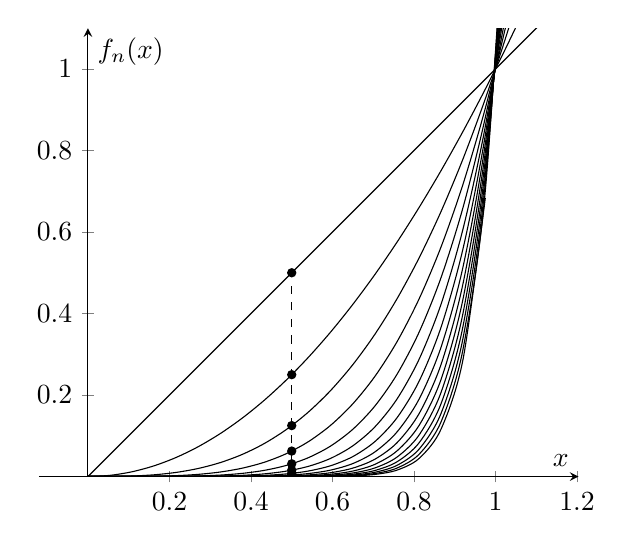
\begin{tikzpicture}
					\pgfmathsetmacro{\xzero}{.5}
					\begin{axis} [
						xlabel={$x$},ylabel={$f_n(x)$},
						axis lines=middle,
						axis equal,
						ymax = 1.1,
						legend pos = outer north east
					]
						\pgfplotsinvokeforeach{1,2,...,15} {
							% Restricting y fixes spurious lines being generated by Adobe Acrobat when printing the graph
							% Also, y domain is a bit bigger than the displayed graph since otherwise the functions wouldn't be properly plotted
							\addplot [smooth, domain=0:1.3, restrict y to domain=0:1.5] {pow(x, #1)};
							% This time around nodes are used instead of \addplot with the * mark
							% in order to control dots size, since bigger dots clutter the image
							\node[circle, fill=black, inner sep=1.2pt] at (\xzero, {pow(\xzero, #1)}) {};
						}

						\draw[dashed] (\xzero, 0) -- (\xzero, \xzero);
					\end{axis}
				\end{tikzpicture}
			}
			\caption{$x_0 = \frac{1}{2}$}
			\label{fig:conv_punt_grap_05}
		\end{subfigure}
		\begin{subfigure}{.33\textwidth}
			\centering
			\resizebox{\linewidth}{!}{
				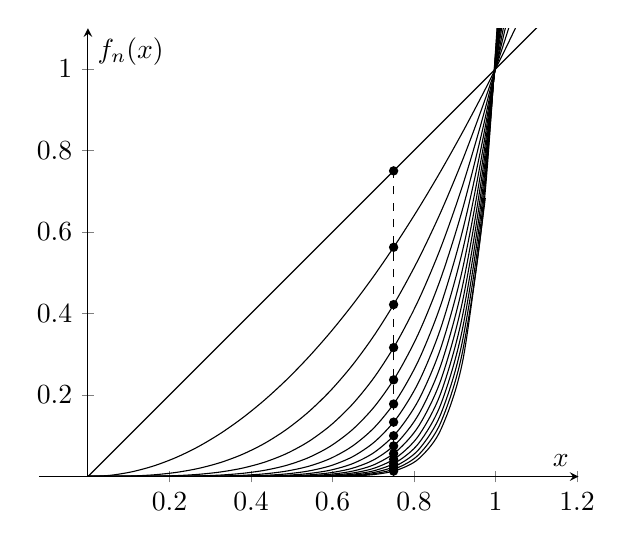
\begin{tikzpicture}
					\pgfmathsetmacro{\xzero}{.75}
					\begin{axis} [
						xlabel={$x$},ylabel={$f_n(x)$},
						axis lines=middle,
						axis equal,
						ymax = 1.1,
						legend pos = outer north east
					]
						\pgfplotsinvokeforeach{1,2,...,15} {
							% Restricting y fixes spurious lines being generated by Adobe Acrobat when printing the graph
							% Also, y domain is a bit bigger than the displayed graph since otherwise the functions wouldn't be properly plotted
							\addplot [smooth, domain=0:1.3, restrict y to domain=0:1.5] {pow(x, #1)};
							% This time around nodes are used instead of \addplot with the * mark
							% in order to control dots size, since bigger dots clutter the image
							\node[circle, fill=black, inner sep=1.2pt] at (\xzero, {pow(\xzero, #1)}) {};
						}

						\draw[dashed] (\xzero, 0) -- (\xzero, \xzero);
					\end{axis}
				\end{tikzpicture}
			}
			\caption{$x_0 = \frac{3}{4}$}
			\label{fig:conv_punt_grap_075}
		\end{subfigure}
		\begin{subfigure}{.33\textwidth}
			\centering
			\resizebox{\linewidth}{!}{
				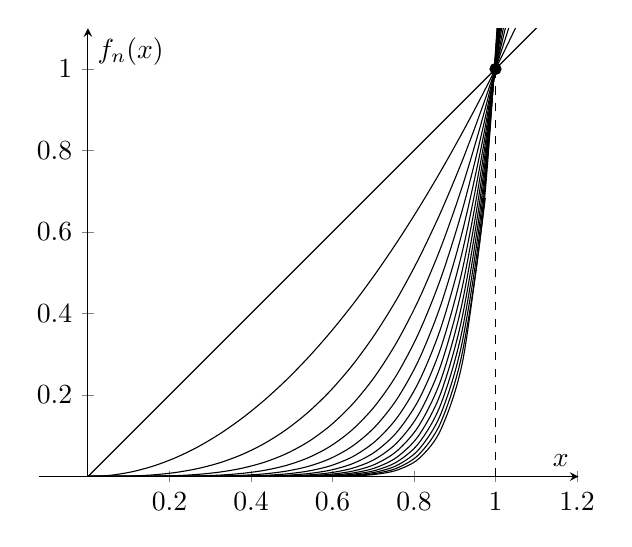
\begin{tikzpicture}
					\pgfmathsetmacro{\xzero}{1}
					\begin{axis} [
						xlabel={$x$},ylabel={$f_n(x)$},
						axis lines=middle,
						axis equal,
						ymax = 1.1,
						legend pos = outer north east
					]
						\pgfplotsinvokeforeach{1,2,...,15} {
							% Restricting y fixes spurious lines being generated by Adobe Acrobat when printing the graph
							% Also, y domain is a bit bigger than the displayed graph since otherwise the functions wouldn't be properly plotted
							\addplot [smooth, domain=0:1.3, restrict y to domain=0:1.5] {pow(x, #1)};
						}

						\addplot [color=black, only marks, mark=*] coordinates {(\xzero, \xzero)};
						\draw[dashed] (\xzero, 0) -- (\xzero, \xzero);
					\end{axis}
				\end{tikzpicture}
			}
			\caption{$x_0 = 1$}
			\label{fig:conv_punt_grap_1}
		\end{subfigure}
		\caption{Si vede che, al crescere di $n$, le $f(x_0)$ convergono a $0$ (in \ref{fig:conv_punt_grap_05} e \ref{fig:conv_punt_grap_075}) o $1$ (in \ref{fig:conv_punt_grap_1})}
	\end{figure}
\end{observation}

\begin{example}
	\label{ex:1_over_n_sin_x_punt_conv}
	La successione di Funzioni con $x \in A \equiv \R$
	\[f_n(x)=\frac{1}{n} \sin(x)\]
	è puntualmente convergente a $0$ su tutto il dominio delle $f_n$, cioè $f_n \pconvarrow 0$ su $B = A = \R$, infatti:
	\[
		\lim\limits_{n \to \infty} f_n(x) = \lim\limits_{n \to \infty} \frac{1}{n} \sin(x) = 0 \quad \forall x \in A
	\]
\end{example}
\begin{example}
	La successione
	\[f_n(x)=e^{nx}\]
	\begin{center}
		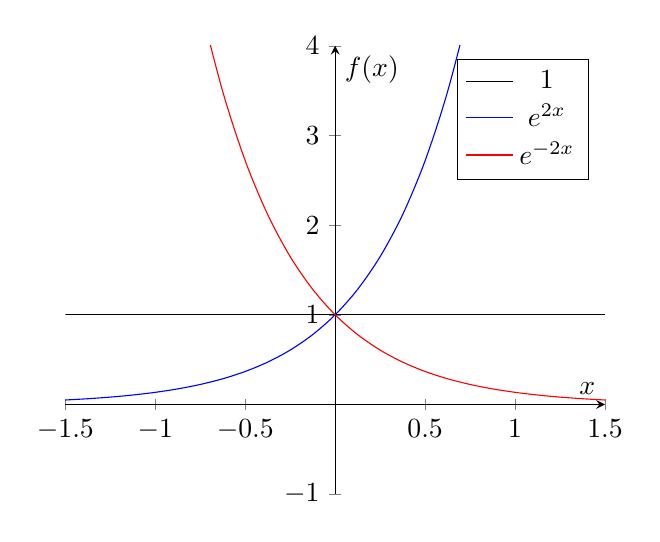
\begin{tikzpicture}
			\begin{axis}[
					xlabel={$x$},ylabel={$f(x)$},
					axis lines=middle,
					domain=-1.5:1.5,
					ymin=-1,ymax=4,
					legend pos = north east
				]
				\addplot[smooth] {1};
				\addlegendentry{$1$}
				\addplot[blue, smooth] {e^(2*x)};
				\addlegendentry{$e^{2x}$}
				\addplot[red, smooth] {e^(-2*x)};
				\addlegendentry{$e^{-2x}$}
			\end{axis}
		\end{tikzpicture}
	\end{center}
	Ha questo comportamento
	\[
		\lim\limits_{n \to \infty} e^{nx} =
		\begin{cases}
			\begin{array}{ll}
				0 & x<0\\
				1 & x=0\\
				\infty & x>0
			\end{array}
		\end{cases}
	\]
	Dunque
	\[f_n \pconvarrow f\quad \text{ su } B = \intervalopcl{-\infty}{0}\]
\end{example}

\begin{proposition}
	\label{prop:conv_punt_lim_succ}
	Siano $B \subseteq A \subseteq \R$, $\brackets{f_n:\; n \in \N}$ una \textbf{Successione di Funzioni} con $f_n:\; A \to \R$ e $f:\; B \to \R$. Allora
	\[
		f_n \pconvarrow f \text{ su } B \text{ per } n \to +\infty
		\quad \iff \quad
		\begin{cases}
			\forall \varepsilon > 0 \quad \forall x \in B\\
			\exists \nu \in \N:\; \forall n > \nu \quad \abs{f_n(x) - f(x)} \leq \varepsilon
		\end{cases}
	\]
	\begin{proof}
		Da \fullref{def:succ_punt_conv} si sa che
		\[f(x) = \lim\limits_{n \to +\infty} f_n(x) \qquad \forall x \in B\]
		Dunque, applicando la \fullref{def:lim_succ}
		\[
			\forall \varepsilon > 0 \quad \exists\nu\in\N:\; \forall n > \nu \quad d \bigl( f_n(x), f(x) \bigr) < \varepsilon  \qquad \forall x \in B
		\]
		Essendo in $f_n$ e $f$ a valori in $\R$, la $d$ è Metrica Euclidea, dunque
		\[
			\forall \varepsilon > 0 \quad \forall x \in B \quad \exists\nu\in\N:\; \forall n > \nu \quad \abs{f_n(x) - f(x)} < \varepsilon
		\]
		\vspace*{-\baselineskip}
		\begin{note}
			È possibile spostare $\forall x \in B$ "a sinistra dei $:$", in quanto, per definizione di $f$ dalla \fullref{def:succ_punt_conv}, $\forall x \in B \quad f(x) = \lim$, quindi la relazione è sempre valida, a prescindere dalla scelta di $x$.
		\end{note}
	\end{proof}
\end{proposition}
\begin{proposition}
	Siano $B \subseteq A \subseteq \R$, $\brackets{f_n:\; n \in \N}$ una \textbf{Successione di Funzioni} con $f_n:\; A \to \R$ e $F:\; B \to \R$. Allora
	\[
		\sum\limits_{n = 0}^{+\infty} f_n \pconvarrow F \text{ su } B
		\quad \iff \quad
		\begin{cases}
			\forall \varepsilon > 0 \quad \forall x \in B\\
			\exists \nu \in \N:\; \forall n > \nu \quad \abs{\sum\limits_{n = 0}^{k} f_n(x) - F(x)} \leq \varepsilon
		\end{cases}
	\]
	\begin{proof}
		Analoga alla \fullref{prop:conv_punt_lim_succ} ricordando la definizione di $F$ in \fullref{def:serie}.
	\end{proof}
\end{proposition}

\begin{proposition}[Metaproposizione sulle Proprietà delle Successioni]
	Sia $f_n:\; A \to \R$, $B \subseteq A \subseteq \R$, $f:\; B \to \R$\\
	Se $f_n \pconvarrow f$ su $B$ e se $f_n$ ha la proprietà $P$, allora la funzione limite puntuale $f$ ha a sua volta la proprietà $P$.
	\begin{note}
		La continuità (e quindi anche la derivabilità) non è una proprietà che passa alla funzione limite, come visto in \fullref{ex:conv_succ_xn}, dove la $f$ ha un punto di discontinuità in $x = 1$.
	\end{note}
	\begin{proof}
		Verrà svolta per le singole proprietà.
	\end{proof}
\end{proposition}
\begin{exercise}
	\label{ex:dim_prop_lim_conv_punt}
	Enunciare rigorosamente e dimostrare:
	\begin{enumerate}
		\item Il limite puntuale della somma (prodotto, combinazione lineare) di due successioni di funzioni è la somma (prodotto, combinazione lineare) delle funzioni limiti puntuali
		\item \label{itm:prop_lim_punt_non_neg} Il limite puntuale di una successione di funzioni non negative è una funzione non negativa
		\item \label{itm:prop_lim_punt_monotonia} Il limite puntuale di una successione di funzioni debolmente/strettamente crescenti/decrescenti è una funzione debolmente crescente/decrescente
		\item Il Criterio di Cauchy (da \fullref{def:succ_cau}) per la convergenza puntuale di serie e successioni
		\item Se la serie $\sum\limits_{n = 0}^{+\infty} f_n(x)$ converge puntualmente in un insieme $B$, allora $f_n \pconvarrow 0$ su $B$
	\end{enumerate}
	\begin{solution}~
		\renewcommand\qedsymbol{$\square$} % To restore the default empty square for the proof environments below
		\begin{enumerate}
			\item[\ref{itm:prop_lim_punt_non_neg}.]
				Sia $f_n:\; A \to \R$, $B \subseteq A \subseteq \R$ e $f:\; B \to A$\\
				Se $f_n \pconvarrow f$ su $B$ e se $f_n$ è non negativa su $B$, cioè $f_n \geq 0$, allora il limite puntuale $f$ è non negativo, $f \geq 0$, su $B$.
				\begin{proof}
					Da \fullref{def:succ_punt_conv}, si sa che
					\[f(x) = \lim\limits_{n \to \infty} f_n(x) \quad \forall x \in B\]
					Ma $f_n$ è, per ipotesi, una successione di valori non negativi, quindi il limite esiste ed è non negativo.

					La dimostrazione è analoga per funzioni non positive.
				\end{proof}
			\item[\ref{itm:prop_lim_punt_monotonia}.]
				Sia $f_n:\; A \to \R$, $B \subseteq A \subseteq \R$ e $f:\; B \to A$\\
				Se $f_n \pconvarrow f$ su $B$ e se $f_n$ è debolmente crescente su $B$, allora il limite puntuale $f$ è debolmente crescente su $B$.
				\begin{proof}
					Il fatto che $f_n$ sia debolmente crescente su $B$ implica che
					\[\forall x_1, x_2 \in B \quad x_1 \leq x_2 \implies f_n(x_1) \leq f_n(x_2)\]
					Con $n \to \infty$, essendo nell'insieme $B$, si ha che $f(x_1) \leq f(x_2)$ per definizione di $f$ da \fullref{def:succ_punt_conv}.

					La dimostrazione è analoga per funzioni debolmente decrescenti e strettamente/debolmente crescenti.
					\let\qed\relax % In order to avoid having two squares, hide the innermost one
				\end{proof}
			% TODO remaining points
			\vspace*{-2\baselineskip} % To remove the whitespace due to enumerate environment
		\end{enumerate}
	\end{solution}
\end{exercise}
\begin{observation}
	In riferimento al punto \ref{itm:prop_lim_punt_non_neg} dell'\fullref{ex:dim_prop_lim_conv_punt}, è necessario sottolineare come non sia invece possibie avere certezze sulla \textbf{stretta} positività/negatività del limite puntuale di una successione di funzioni strettamente positive/negative.\\
	Ad esempio, $-\frac{e^x}{n}$ con $x \in \intervalclop{0}{1}$ è strettamente negativa, ma il limite puntuale è costante $0$.
\end{observation}
\begin{observation}
	In riferimento al punto \ref{itm:prop_lim_punt_monotonia} dell'\fullref{ex:dim_prop_lim_conv_punt}, è necessario sottolineare come non sia invece possibie avere certezze sulla \textbf{stretta} crescenza/decrescenza del limite puntuale.\\
	Come esempio, vedasi \fullref{ex:conv_succ_xn} in cui si studia la successione strettamente crescente $x^n$, il cui limite puntuale è però costante (dunque non \textbf{strettamente} crescente) in $B = \intervalclop{0}{1}$.
\end{observation}
\begin{exercise}
	Verificare che il limite puntuale di funzoni \textbf{Continue} e \textbf{Derivabili}, quando esiste, può essere una funzione \textbf{Continua} e \textbf{non Derivabile}.\\
	Considerare ad esempio $f_n:\; \R \to \R$ data da $f_n(x) = \sqrt{x^2 + \frac{1}{n}}$ visibile in \cref{fig:fn_sqrt_x2_1_over_n}.
	% TODO solution
\end{exercise}
\begin{exercise}
	Verificare che il limite puntuale di funzoni \textbf{Continue} e \textbf{Derivabili}, quando esiste, può essere una funzione \textbf{non Continua}.\\
	Considerare ad esempio $f_n:\; \R \to \R$ data da $f_n(x) = \arctan(nx)$ visibile in \cref{fig:fn_sqrt_x2_1_over_n}.
	% TODO solution
\end{exercise}
\begin{exercise}
	Determinare, se possibile, sotto quali ipotesi sulla funzione $f:\; \R \to \R$ le seguenti successioni di funzioni risultano Puntualmente Convergenti:
	\begin{alignat*}{2}
		f_n(x) &= f(x) + n \hspace*{.35\linewidth} & f_n(x) &= f(x + n)\\
		f_n(x) &= f(x) + \frac{1}{n} & f_n(x) &= f(x + \frac{1}{n})\\
		f_n(x) &= nf(x) & f_n(x) &= \frac{f(x)}{n}\\
		f_n(x) &= f(nx) & f_n(x) &= f(\frac{x}{n})
	\end{alignat*}
\end{exercise}

\cbstart
\begingroup
% This group is used to alter equation numbering, since there are equations outside environments
\renewcommand\theequation{\arabic{section}.\arabic{equation}}
\setcounter{equation}{0} % Reset counter to fix numbering for equation outside theorem envs
\subsection{L'Insufficienza della Convergenza Puntuale}\label{sect:insuff_conv_punt}
La Convergenza Puntuale si può rivelare insufficiente per diverse ragioni, tra cui:
\begin{itemize}
	\item
		Può spesso esser comodo utilizzare una successione $f_n$ convergente puntualmente a $f$ nel caso in cui $f$ non sia ottenibile in modo esplicito (ad esempio nella soluzione di un'equazione differenziale). Però, come visto in \fullref{ex:conv_succ_xn}, la convergenza puntuale non trasferisce necessariamente proprietà come Continuità, Limitatezza o Derivabilità alla funzione limite puntuale.
		La successione $f_n = x^n$ di \fullref{ex:conv_succ_xn}, ad esempio, è formata da funzioni $\in \cntclass{\infty}(\intervalclose{0}{1}; \R)$, però la funzione limite puntuale
		\[
			f =
			\begin{cases}
				\begin{array}{ll}
					0 & \text{se } x \in \intervalopen{-1}{1}\\
					1 & \text{se } x = 1
				\end{array}
			\end{cases}
		\]
		non è né continua né, dunque, derivabile nello stesso intervallo.
		\begin{figure}[H]
			\begin{subfigure}{.49\textwidth}
				\centering
				\resizebox{\linewidth}{!}{
					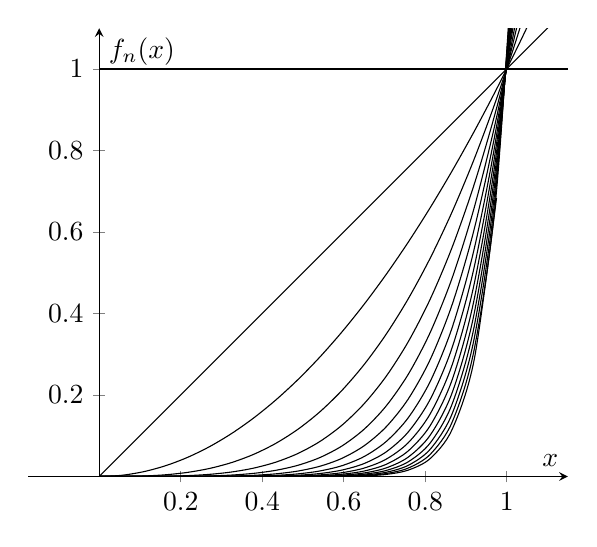
\begin{tikzpicture}
						\begin{axis} [
							xlabel={$x$},ylabel={$f_n(x)$},
							axis lines=middle,
							axis equal,
							% xmax is used only to force same width to both graphs, thus having same height when resized
							ymax = 1.1, xmax = 1.15,
							legend pos = outer north east
						]
							\pgfplotsinvokeforeach{0,1,...,15} {
								% Restricting y fixes spurious lines being generated by Adobe Acrobat when printing the graph
								% Also, y domain is a bit bigger than the displayed graph since otherwise the functions wouldn't be properly plotted
								\addplot [smooth, domain=0:1.3, restrict y to domain=0:1.5] {pow(x, #1)};
							}
						\end{axis}
					\end{tikzpicture}
				}
				\caption{$f_n(x) = x^n \quad 0 \leq n \leq 15$}
			\end{subfigure}
			\begin{subfigure}{.49\textwidth}
				\centering
				\resizebox{\linewidth}{!}{
					\begin{tikzpicture}
						\begin{axis} [
							xlabel={$x$},ylabel={$f(x)$},
							axis lines=middle,
							axis equal,
							% xmax is used only to force same width to both graphs, thus having same height when resized
							ymax = 1.1, xmax = 1.15,
							legend pos = outer north east
						]
							\addplot [smooth, line width=2pt, domain=0:1] {0};
							\addplot [color=black, fill=white, only marks, mark=*] coordinates {(1,0)};
							\addplot [color=black, only marks, mark=*] coordinates {(1,1)};
						\end{axis}
					\end{tikzpicture}
				}
				\caption{$f(x) \quad x \in \intervalclose{0}{1}$}
			\end{subfigure}
			\caption{$f_n(x) \in \cntclass{\infty}(\intervalclose{0}{1}; \R)$, mentre la funzione limite puntuale $f$ è discontinua.}
			\label{fig:cont_fn_non_passa_a_f}
		\end{figure}
	\item
		Supponendo di voler calcolare l'integrale
		\begin{equation}
			\label{eq:insuf_conv_punt_int_f}
			\int_a^b f(x) \integrald{x}
		\end{equation}
		Ma con $f$ non integrabile (o magari anche solo $f$ non integrabile in modo elementare). Si cercherebbe dunque di approssimarlo con una successione di integrali tipo
		\begin{equation}
			\label{eq:insuf_conv_punt_int_fn}
			\int_a^b f_n(x) \integrald{x}
		\end{equation}
		Potrebbe venire naturale di prendere una successione $f_n$ Puntualmente Convergente a $f$ e quindi considerare gli integrali delle $f_n$ della \cref{eq:insuf_conv_punt_int_fn} come approssimazioni dell'integrale \cref{eq:insuf_conv_punt_int_f}. Questo ragionamento è però valido solo nel caso in cui valga
		\begin{equation}
			\label{eq:conv_punt_pass_lim_integrale}
			\lim\limits_{n \to +\infty} \int_a^b f_n(x) \integrald{x} = \int_a^b \lim\limits_{n \to +\infty} f_n(x) \integrald{x} = \int_a^b f(x) \integrald{x}
		\end{equation}
		Cioè eseguendo il \textit{passaggio al limite sotto il segno di integrale}, operazione di cui si è già parlato nell'introduzione al \fullref{chap:int_doppi} specificando che, con gli integrali di Riemann, non è affatto scontato sia possibile.\\
		Nel caso della convergenza puntuale non son garantite le iptesi necessarie, dunque non è possibile passare al limite sotto l'integrale, come si vede nel successivo \fullref{ex:conv_punt_no_pass_lim_integrale}.
\end{itemize}
La Convergenza Puntuale presenta le problematiche evidenziate in quanto non si basa su alcun tipo di concetto di \textbf{distanza tra funzioni}. Infatti, ricordando \fullref{def:succ_punt_conv}, avere convergenza puntuale $f_n \pconvarrow f$ su un certo insieme $A$ significa che, fissato un qualsiasi $x_0 \in A$, si ha
\[\lim\limits_{n \to +\infty} d \bigl( f_n(x_0), f(x_0) \bigr) = 0\]
Con $d$ Metrica Euclidea, distanza tra i valori di $f_n$ ed $f$ nel punto $x_0$ precedentemente fissato. In pratica, i valori di $f_n$ e $f$ vengono considerati \textbf{punto per punto} separatamente e la convergenza puntuale non è influenzata da tutti gli altri valori che le funzioni possono assumere in un intorno di $x_0$.
\begin{example}
	\label{ex:conv_punt_no_pass_lim_integrale}
	La successione
	\[
		\funcdef{f_n}{\intervalclose{0}{1}}{\R}{x}{
			\begin{cases}
				\begin{array}{ll}
					0 & \text{se } x \in \brackets{0} \cup \intervalopcl{\frac{1}{n}}{1}\\
					-n^2x + n & \text{se } x \in \intervalopcl{0}{\frac{1}{n}}
				\end{array}
			\end{cases}
		}
	\]
	converge puntualmente alla funzione $f(x) = 0$ su $\intervalclose{0}{1}$. Infatti, essendo $\frac{1}{n} \to 0$ per $n \to +\infty$, un qualsiasi $x \in \intervalclose{0}{1}$ cadrà nell'intervallo $\intervalopcl{\frac{1}{n}}{1}$ in cui $f_n$ è definita essere $0$. Quindi $\lim\limits_{n \to +\infty} f_n(x) = 0$.
	\begin{center}
		\begin{tikzpicture}
			\begin{axis} [
				clip mode = individual,
				xlabel={$x$},ylabel={$f_n(x)$},
				axis lines=middle,
				xmax=1.2, ymax=5.5,
				xtick = {1/2, 1},
				xticklabels = {$\frac{1}{n}$, $1$},
				ytick = {2},
				yticklabels = {$n$}
			]
				\addplot [color=black, only marks, mark=*] coordinates {(0,0)};
				\pgfplotsinvokeforeach{2, 3, 5} {
					\addplot [thick, domain=0:(1/#1)] {-pow(#1, 2)*x + #1};
					\addplot [color=black, fill=white, only marks, mark=*] coordinates {(0,#1)};
				}
				\addplot [line width=2pt, domain=(1/5):1] {0}; % We need only a single line on x axis, the one starting at the smallest 1/n
			\end{axis}
		\end{tikzpicture}
	\end{center}
	Gli integrali delle $f_n$ sono:
	\begin{align*}
		&\int_0^1 f_n(x) \integrald{x} =\\
		&= \int_0^{\frac{1}{n}} \left( -n^2x + n \right)\integrald{x} + \int_{\frac{1}{n}}^1 0 \integrald{x}\\
		&= \left[ -\frac{n^2}{2}x^2 + nx \right]_0^{\frac{1}{n}}\\
		&= -\frac{n^2}{2}\frac{1}{n^2} + n \frac{1}{n}\\
		&= \frac{1}{2}
	\end{align*}
	L'integrale della funzione limite puntuale $f$ sarebbe, ovviamente, $0$, essendo stato dimostrato prima che $f_n \pconvarrow 0$, dunque l'uguaglianza di \cref{eq:conv_punt_pass_lim_integrale} non vale.
\end{example}

\subsection{Distanze tra Funzioni}\label{sect:dist_funz}
La nozione di distanza si basa, generalmente, su una preesistente nozione di "grandezza": stabilito il modo per valutare la grandezza di un ente, è ragionevole ritenere che due oggetti siano tanto più vicini quanto più è "piccola" la differenza tra essi. Cioè la distanza può essere vista come la "grandezza" della differenza (ovviamente, quando è ammessa la differenza tra gli oggetti). Si è vista l'applicazione di questo criterio in molti esempi di \fullref{ex:metriche}.

Dovendo valutare la distanza tra funzioni, è dunque necessario prima stabilire come valutare la "grandezza" delle funzioni stesse.

Quale delle seguenti funzioni ha senso definire "più grande"?
\begin{figure}[H]
	\begin{subfigure}{.49\textwidth}
		\centering
		\resizebox{\linewidth}{!}{
			\begin{tikzpicture}
				\begin{axis} [
					xlabel={$x$},ylabel={$f(x)$},
					axis lines=center,
					axis on top = true,
					axis equal,
					xmin = -4, xmax = 4,
					ymin = -.5, ymax = 6,
					xtick = {-3, 3},
					xticklabels = {$a$, $b$}
				]
					\addplot [name path=f, smooth, domain=-5:5, samples=50] {exp(-10*x^2)*5};
					\path[name path=axis] (\pgfkeysvalueof{/pgfplots/xmin},0) -- (\pgfkeysvalueof{/pgfplots/xmax},0);
					\addplot[black!30] fill between[of=f and axis, soft clip={domain=-3:3}];
				\end{axis}
			\end{tikzpicture}
		}
		\caption{Curva gaussiana}
		\label{pic:grand_funz_gauss}
	\end{subfigure}
	\begin{subfigure}{.49\textwidth}
		\centering
		\resizebox{\linewidth}{!}{
			\begin{tikzpicture}
				\begin{axis} [
					xlabel = $x$, ylabel = {$f(x)$},
					axis lines = center,
					axis on top = true,
					axis equal,
					xmin = -4, xmax = 4,
					ymin = -.5, ymax = 6,
					xtick = {-3, 3},
					xticklabels = {$a$, $b$}
				]
					\addplot [name path=f, smooth, domain=-5:5, samples=50] {-(4/7*x)^2+3};
					\path[name path=axis] (\pgfkeysvalueof{/pgfplots/xmin},0) -- (\pgfkeysvalueof{/pgfplots/xmax},0);
					\addplot[black!30] fill between[of=f and axis, soft clip={domain=-3:3}];
				\end{axis}
			\end{tikzpicture}
		}
		\caption{Parabola rovesciata}
		\label{pic:grand_funz_parab}
	\end{subfigure}
	\caption{Diversi parametri per valutare la "grandezza" di una funzione}
\end{figure}

Ovviamente dipende dall'aspetto che si intende considerare. La \ref{pic:grand_funz_gauss} potrebbe essere "più grande" perché ha massimo maggiore rispetto a \ref{pic:grand_funz_parab}, che però d'altro canto ha una maggiore area sottesa.

Questi erano solo due esempi di "grandezza" di una funzione, definiti con le seguenti metriche
\[
	\norm{f}_{\cntclass{0}} = \sup\limits_{x \in \intervalclose{a}{b}} \abs{f(x)}
	\qquad\qquad\qquad\qquad\qquad
	\norm{f}_1 = \int_a^b \abs{f(x)} \integrald{x}
\]
Quella di sinistra è la \textbf{Norma Infinito} o \textbf{Norma del} $\boldsymbol{\sup}$, mentre a destra \textbf{Norma Indice} $\boldsymbol{1}$. In aggiunta, si definisce anche la \textbf{Norma Indice} $\boldsymbol{2}$, che sarà usata in \fullref{sect:conv_quadr}:
\[\norm{f}_2 = \sqrt{ \int_a^b \left[f(x)\right]^2 \integrald{x} }\]

Le distanze indotte dalle seguenti norme saranno dunque
\[
	d_{\cntclass{0}} (f, g) = \norm{f - g}_{\cntclass{0}}
	\qquad\qquad\qquad
	d_1 = \norm{f - g}_1
	\qquad\qquad\qquad
	d_2 = \norm{f - g}_2
\]
E si parla di \textbf{Distanza Infinito} (o \textbf{Distanza del} $\boldsymbol{\sup}$), \textbf{Distanza Indice} $\boldsymbol{1}$ e \textbf{Distanza Indice} $\boldsymbol{2}$.

\begin{figure}[H]
	\begin{subfigure}{.49\textwidth}
		\centering
		\resizebox{\linewidth}{!}{
			\begin{tikzpicture}[
				declare function = {
					f(\x) = sqrt(\x)*(sin(deg(\x))+1);
					g(\x) = sqrt(\x);
				},
				> = stealth
			]
			\begin{axis} [
				xlabel={$x$},ylabel={$y$},
				axis lines=middle,
				ymax=9,
				legend style = {at={(.1,.95)}, anchor = north west}
			]
				\addplot [thick, name path=f, smooth, domain=0:10, samples=50] {f(x)};
				\addlegendentry{$f$};
				\addplot [color=blue, thick, name path=g, smooth, domain=0:10, samples=100] {g(x)};
				\addlegendentry{$g$};
				\pgfplotsinvokeforeach{.25,.5,...,10} {
					\draw[thin, black!60] (#1, {f(#1)}) -- (#1, {g(#1)});
				}
				% Mark thicker the sup
				\draw[thick] (8, {g(8)}) -- (8,{f(8)});
				\node (text_sup_dist) [align=center] at (6.5,8) {$\sup \abs{f(x) - g(x)}$};
				\draw[thin, ->, shorten >=4pt] (text_sup_dist.south) to [out=-90, in=90](8,{f(8)});

				\addplot[brown!30] fill between[of=f and g];
				\addlegendentry{$d_1$};
			\end{axis}
		\end{tikzpicture}
		}
		\caption{Significato grafico di\\Distanza Infinito e Distanza Indice $1$}
	\end{subfigure}
	\begin{subfigure}{.49\textwidth}
		\centering
		\resizebox{\linewidth}{!}{
			\begin{tikzpicture}[
				declare function = {
					f(\x) = sqrt(\x)*(sin(deg(\x))+1);
					g(\x) = sqrt(\x);
				},
				> = stealth
			]
				\begin{axis} [
					xlabel={$x$},ylabel={$y$},
					axis lines=middle,
					axis on top = true,
					ymax=9,
					legend style = {at={(.1,.95)}, anchor = north west}
				]
					\addplot [thick, name path=f, smooth, domain=0:10, samples=100] {(f(x)-g(x))^2};
					\addlegendentry{$\bigl[ f(x) - g(x) \bigr]^2$};
					\path[name path=axis] (\pgfkeysvalueof{/pgfplots/xmin},0) -- (\pgfkeysvalueof{/pgfplots/xmax},0);
					\addplot[brown!30] fill between[of=f and axis];
					\addlegendentry{$d_2$};
				\end{axis}
			\end{tikzpicture}
		}
		\caption{Significato grafico (a meno della radice) di\\Distanza Indice $2$}
	\end{subfigure}
\end{figure}
\cbend
\endgroup

\subsection{Convergenza Uniforme}\label{sect:conv_unif}
Si chiama convergenza uniforme la convergenza di una Successione rispetto alla distanza $d_{\cntclass{0}}$.

\begin{definition}[Successione Uniformemente Convergente]
	\label{def:succ_unif_conv}
	Siano $B \subseteq A \subseteq \R$, $\brackets{f_n:\; n \in \N}$ una \textbf{Successione di Funzioni} e $f_n:\; A \to \R$.\\
	La Successione $f_n$ è \textbf{Uniformemente Convergente} su $B$ se esiste la \textbf{Funzione Limite Uniforme} $f:\; B \to \R$ tale che:
	\[\lim\limits_{n \to +\infty} \sup\limits_{B} \abs{f_n(x) - f(x)} = 0\]
	\begin{note}
		Nella \fullref{def:succ_punt_conv} la $f$ associava ogni punto al valore a cui convergeva la successione in quel punto.\\
		In questo caso invece la $f$ è una funzione \textit{tale per cui} la distanza massima (per via del $\sup$ di $d_{\cntclass{0}}$) tra $f_n$ e $f$ è $0$. Questo vuol dire che la funzione "coincide con la $f_n$ su tutto $B$", in quel senso \textit{Uniformemente}. Vedasi \fullref{obs:diff_conv_unif_e_conv_punt}.
	\end{note}
	La convergenza uniforme su $B$ della successione $f_n$ verso $f$ è indicata con
	\[f_n \uconvarrow f \text{ su } B\]
\end{definition}
\begin{definition}[Serie Uniformemente Convergente]
	Siano $B \subseteq A \subseteq \R$, $\brackets{f_n:\; n \in \N}$ una \textbf{Successione di Funzioni} e $f_n:\; A \to \R$.\\
	La \textbf{Serie} $s = \sum\limits_{n = 0}^{+\infty} f_n(x)$ associata alla Successione $f_n$ è \textbf{Uniformemente Convergente} su $B$ se esiste la \textbf{Funzione Limite Uniforme} $F:\; B \to \R$ tale che:
	\[\lim\limits_{n \to +\infty} \sup\limits_{B} \abs{\sum\limits_{n = 0}^{+\infty} f_n(x) - F(x)} = 0\]
\end{definition}

\begin{example}~
	\begin{figure}[H]
		\centering
		\begin{tikzpicture}[
			declare function = {
				f_n(\x) = sqrt(\x)*(1/4*(sin(deg(\x))+4));
				f(\x) = sqrt(\x);
			},
			> = stealth
		]
			\begin{axis} [
				xlabel={$x$},ylabel={$y$},
				axis lines=middle,
				axis on top = true,
				ymax=9,
				legend style = {at={(.1,.95)}, anchor = north west}
			]
				\addplot [thick, name path=f_n, smooth, domain=0:10, samples=50] {f_n(x)};
				\addlegendentry{$f_n$};
				\addplot [color=blue, thick, smooth, domain=0:10, samples=100] {f(x)};
				\addlegendentry{$f$};
				\addplot [color=red, name path=f_plus, smooth, domain=0:10, samples=100] {f(x) + 1.2};
				\addlegendentry{$f + \varepsilon$};
				\addplot [color=green, name path=f_minus, smooth, domain=0:10, samples=100] {f(x) - 1.2};
				\addlegendentry{$f - \varepsilon$};
				\pgfplotsinvokeforeach{.25,.5,...,10} {
					\draw[thin, black!60] (#1, {f_n(#1)}) -- (#1, {f(#1)});
				}
				% Mark thicker the sup
				\draw[thick] (8, {f(8)}) -- (8,{f_n(8)});
				\node (text_sup_dist) [align=center] at (7,6.5) {$\sup \abs{f_n(x) - f(x)} < \varepsilon$};
				\draw[thin, ->, shorten >=2pt] (text_sup_dist.south) to [out=-90, in=90](8,{f_n(8)});

				\addplot[brown!30, forget plot] fill between[of=f_plus and f_minus];
			\end{axis}
		\end{tikzpicture}
		\caption{Significato grafico della Convergenza Uniforme\\Come si vedrà in {\protect\fullref{prop:conv_unif_lim_succ}}}
	\end{figure}
\end{example}

\begin{observation}
	\label{obs:dist_conv_unif}
	La convergenza uniforme equivale alla convergenza rispetto alla distanza $d_{\cntclass{0}}(f,g)=\sup\limits_{x\in A}\abs{g(x)-f(x)}$ ogniqualvolta questa distanza sia definita. La definizione di $d_{\cntclass{0}}(f,g)$ come \textit{distanza} è dimostrata in \hyperref[ex:dim_dist_conv_unif]{\fullref*{ex:metriche}}\\
	% NOTE The \fullref command was not used on purpose to point this link straight to the right part of the aforementioned exercise
	La $d_{\cntclass{0}}(f,g)$ può anche essere definita attraverso la \textbf{norma} $\norm{k}_{\cntclass{0}}=\sup\limits_{x\in A}\abs{k}$ con $k = f-g$ in quanto, in $\R$ norma e valore assoluto coincidono.
\end{observation}
\begin{example}
	Come già visto in \fullref{ex:1_over_n_sin_x_punt_conv}, la Successione di Funzioni con $x \in A \equiv \R$
	\[f_n(x) = \frac{1}{n} \sin(x)\]
	è $f_n \pconvarrow 0$ su $A$. Questa stessa Successionione è anche Uniformemente Convergente su $A$, infatti:
	\[
		\lim\limits_{n \to +\infty} \sup\limits_{A} \abs{f_n(x) - 0} =
		\lim\limits_{n \to +\infty} \sup\limits_{A} \abs{\frac{1}{n} \sin(x)}
	\]
	Osservando che $\abs{a \cdot \sin(x)} \leq \abs{a}$, si può conclduere
	\[
		\lim\limits_{n \to +\infty} \sup\limits_{\R} \abs{\frac{1}{n} \sin(x)} \leq
		\lim\limits_{n \to +\infty} \frac{1}{n}=0
	\]
	Allora $f_n \uconvarrow f$ su $A$
\end{example}

\begin{exercise}
	\label{ex:dim_dist_inf}
	Sia $K \in \R$ un \textbf{Compatto}. Verificare che:
	\begin{enumerate}
		\item $\norm{\;\cdot\;}_{\cntclass{0}}$ è una norma su $\cntclass{0}(K; \R)$
		\item \label{itm:dim_dist_inf_dist} $d_{\cntclass{0}}$ è una distanza su $\cntclass{0}(K; \R)$
		\item La convergenza rispetto alla distanza $d_{\cntclass{0}}$ equivale alla convergenza uniforme su $K$
	\end{enumerate}
	\begin{solution}~
		\begin{enumerate}
			\item[\ref{itm:dim_dist_inf_dist}.] Dimostrata in \hyperref[ex:dim_dist_conv_unif]{\fullref*{ex:metriche}}
			% NOTE The \fullref command was not used on purpose to point this link straight to the right part of the aforementioned exercise
		\end{enumerate}
		% TODO remaining points proof
	\end{solution}
\end{exercise}
\begin{proposition}
	\label{prop:conv_unif_lim_succ}
	Siano $B \subseteq A \subseteq \R$, $\brackets{f_n:\; n \in \N}$ una \textbf{Successione di Funzioni} e $f_n:\; A \to \R$. Sia $f:\; B \to \R$ una funzione:
	\[
		f_n \uconvarrow f \text{ su } B \text{ per } n \to +\infty
		\quad \iff \quad
		\begin{cases}
			\forall \varepsilon > 0 \quad \exists \nu \in \N:\\
			\forall n > \nu \quad \forall x \in B \quad \abs{f_n(x) - f(x)} \leq \varepsilon
		\end{cases}
	\]
	\begin{solution}
		Da \fullref{def:succ_unif_conv} si sa che
		\[\lim\limits_{n \to +\infty} \sup\limits_{B} \abs{f_n(x) - f(x)} = 0\]
		Dunque, applicando la \fullref{def:lim_succ}
		\[
			\forall \varepsilon > 0 \quad \exists\nu\in\N:\; \forall n > \nu \quad d \bigl( \abs{f_n(x) - f(x)}, 0 \bigr) < \varepsilon  \qquad \forall x \in B
		\]
		Essendo in $f_n$ e $f$ a valori in $\R$, la $d$ è Metrica Euclidea, dunque
		\[
			\forall \varepsilon > 0 \quad \exists\nu\in\N:\; \forall n > \nu \quad \forall x \in B \quad \bigl| \abs{f_n(x) - f(x)} - 0 \bigr| < \varepsilon
		\]
		\begin{note}
			A differenza di quanto fatto in \fullref{prop:conv_punt_lim_succ}, non è possibile spostare $\forall x \in B$ "a sinistra dei $:$". La scelta di $x$ non è \textit{"a prescindere"}, ma subordinata alla scelta di $\varepsilon$ e $\nu$. Dato dunque un certo $\nu$, allora, per ogni $n$ e $x$, vale il limite. Vedasi \fullref{obs:diff_conv_unif_e_conv_punt}.
		\end{note}
	\end{solution}
\end{proposition}
\begin{proposition}
	Siano $B \subseteq A \subseteq \R$, $\brackets{f_n:\; n \in \N}$ una \textbf{Successione di Funzioni} con $f_n:\; A \to \R$ e $F:\; B \to \R$. Allora
	\[
		\sum\limits_{n = 0}^{+\infty} f_n \uconvarrow F \text{ su } B
		\quad \iff \quad
		\begin{cases}
			\forall \varepsilon > 0 \quad \exists \nu \in \N:\\
			\forall n > \nu \quad \forall x \in B \quad \abs{\sum\limits_{n = 0}^{k} f_n(x) - F(x)} \leq \varepsilon
		\end{cases}
	\]
	\begin{proof}
		Analoga alla \fullref{prop:conv_unif_lim_succ} ricordando la definizione di $F$ in \fullref{def:serie}.
	\end{proof}
\end{proposition}
\begin{observation}
	\label{obs:diff_conv_unif_e_conv_punt}
	La differenza tra \fullref{prop:conv_unif_lim_succ} e \fullref{prop:conv_punt_lim_succ} (e rispettive proposizioni sulle Serie) giustifica il fatto che la continuità non passi alla Funzione Limite Puntuale, come spiegato in \fullref{sect:insuff_conv_punt}.

	Infatti qui $\nu$ dipende solo dalla scelta di $\varepsilon$ e le $x$ "si guardano tutte insieme", nella Convergenza Puntuale invece $\nu$ dipendeva, oltre che dalla $\varepsilon$, anche dalla $x$. Questo portava ad osservare le $x$ una alla volta.
\end{observation}
\begin{corollary}[Relazione tra Convergenza Uniforme e Puntuale]
	\label{coro:if_unif_conv_then_punt_conv}
	Siano $B \subseteq A \subseteq \R$ e $\brackets{f_n:\; n \in \N}$ una \textbf{Successione di Funzioni} e $f_n:\; A \to \R$. Sia $f:\; B \to \R$ una funzione
	\[f_n \uconvarrow f \text{ su } B \quad \implies \quad  f_n \pconvarrow f \text{ su } B\]
	\vspace*{-\baselineskip}
	\begin{note}
		Questo significa che la Convergenza Uniforme ha tutte le proprietà della Convergenza Puntuale.
	\end{note}
	\begin{note}
		L'implicazione inversa non è possibile, come si vede in \fullref{ex:conv_punt_nimplies_conv_unif}.
	\end{note}
	\begin{proof}
		Da \fullref{prop:conv_unif_lim_succ}  si sa che valgono condizioni analoghe, ma più restrittive, rispetto a quelle di \fullref{prop:conv_punt_lim_succ} (vedere note alle due Proposizioni), dunque sicuramente è valida l'implicazione $\impliedby$ di \fullref{prop:conv_punt_lim_succ}.
	\end{proof}
\end{corollary}
\begin{example}[La Convergenza Puntuale non implica Convergenza Uniforme]
	\label{ex:conv_punt_nimplies_conv_unif}
	Sia $f_n:\; \R \to \R$ data da $f_n(x) = x^n$, allora:
	\[
		f_n \pconvarrow f \text{ su } \intervalopcl{-1}{1}
		\qquad \text{dove} \qquad
		f(x) = \begin{cases}
			\begin{array}{ll}
				0 & \text{per } x \in \intervalopen{-1}{1}\\
				1 & \text{per } x = 1
			\end{array}
		\end{cases}
	\]
	Ma su $\intervalopcl{-1}{1}$ non c'è convergenza uniforme e nemmeno su $\intervalopen{-1}{1}$.
\end{example}
\begin{exercise}
	È possibile costruire una successione di funzioni $f_n$ uniformemente convergenti ad una successione $f$ non limitata?
	\begin{solution}
		No, perché, come visto in \fullref{coro:if_unif_conv_then_punt_conv} $f_n \uconvarrow f \implies f_n \pconvarrow f$, ma per \fullref{def:succ_punt_conv} $\nexists$ successione puntualmente convergente a $f$ non limitata.
		% TODO controllare soluzione
	\end{solution}
\end{exercise}
\begin{exercise}
	Determinare, se possibile, sotto quali ipotesi sulla funzione $f:\; \R \to \R$ le seguenti successioni di funzioni sono Uniformemente Convergenti:
	\begin{alignat*}{2}
		f_n(x) &= f(x) + n \hspace*{.35\linewidth} & f_n(x) &= f(x + n)\\
		f_n(x) &= f(x) + \frac{1}{n} & f_n(x) &= f(x + \frac{1}{n})\\
		f_n(x) &= nf(x) & f_n(x) &= \frac{f(x)}{n}\\
		f_n(x) &= f(nx) & f_n(x) &= f(\frac{x}{n})
	\end{alignat*}
\end{exercise}
\begin{definition}[Successione di Funzioni di Cauchy per la Convergenza Uniforme]
	\label{def:succ_funz_cau}
	Siano $B \subseteq A \subseteq \R$, $\brackets{f_n:\; n \in \N}$ una \textbf{Successione di Funzioni} e $f_n:\; A \to \R$
	\begin{center}
		La Successione $\brackets{f_n:\; n \in \N}$ soddisfa alla \textbf{Condizione di Cauchy}\\
		per la \textbf{Convergenza Uniforme} su $B$\\
		$\bydef$\\
		$
			\forall \varepsilon > 0 \quad \exists \nu \in \N: \quad \forall n, m > \nu \quad \forall x \in B %
			\qquad \text{vale} \qquad \abs{f_n(x) - f(x)} < \varepsilon
		$
	\end{center}
\end{definition}
\begin{proposition}
	\label{prop:in_compat_succ_funz_cau_corrisp_a_succ_cau}
	Nel caso in cui $B$ sia \textbf{Compatto}, la \fullref{def:succ_funz_cau} coincide alla \fullref{def:succ_cau}.
	\begin{proof}
		Dalla \fullref{def:compatto}, si sa che ogni successione ammette una sottosuccessione avente limite in $B$, dunque si arriva ad avere la distanza $d \left( \lim\limits_{n \to +\infty}f_n(x), f(x) \right)$ tra due elementi di $K$.
	\end{proof}
\end{proposition}
\begin{definition}[Serie di Funzioni di Cauchy per la Convergenza Uniforme]
	Siano $B \subseteq A \subseteq \R$, $\brackets{f_n:\; n \in \N}$ una \textbf{Successione di Funzioni} e $f_n:\; A \to \R$
	\begin{center}
		La Serie $\sum\limits_{n = 0}^{+\infty}$ associata alla Successione $f_n$ soddisfa alla \textbf{Condizione di Cauchy}\\
		per la \textbf{Convergenza Uniforme} di serie su $B$\\
		$\bydef$\\
		$
			\forall \varepsilon > 0 \quad \exists \nu \in \N:\; \forall n, m > \nu \quad \forall x \in B %
			\qquad \text{vale} \qquad \abs{ \sum\limits_{k = n}^{m} f_k(x) } < \varepsilon
		$
	\end{center}
\end{definition}

\begin{proposition}
	\label{prop:succ_funz_cau_allora_esiste_f_conv_unif}
	Siano $B \subseteq A \subseteq \R$, $\brackets{f_n:\; n \in \N}$ una \textbf{Successione di Funzioni} e $f_n:\; A \to \R$
	\[
		\left.
			\begin{array}{c}
				\text{La Successione } f_n \text{ soddisfa}\\
				\text{alla \textbf{Condizione di Cauchy}}\\
				\text{per la \textbf{Convergenza Uniforme} su } B
			\end{array}
		\right\}
		\implies
		\begin{cases}
			\begin{array}{c}
				\text{Esiste una funzione}\\
				f:\; B \to \R\\
				\text{tale che } f_n \uconvarrow f \text{ su } B
			\end{array}
		\end{cases}
	\]
	\begin{proof}
		Se la successione $\brackets{f_n:\; n \in \N}$ soddisfa la \fullref{def:succ_funz_cau} su $B$\\
		$\implies$ ogni successione $\brackets{f_n(x):\; n \in \N},\; \forall x \in B$, è di Cauchy in $\R$\\
		$\implies$ essendo $\R$ Completo, per \fullref{def:completo} ogni successione
		\[\brackets{f_n(x):\; n \in \N},\; \forall x \in B\]
		avrà limite in $\R$. Sia posta ora $f(x)$ la funzione che associa ad ogni $x$ il limite della $f_n(x)$.

		Si verifica che $f$ è la Funzione Limite Uniforme della successione $\brackets{f_n(x):\; n \in \N}$ su $B$. Infatti, posto $\varepsilon > 0$, sia $\nu \in \N$ tale che $\sup\limits_{B} \abs{f_h - f_k} < \varepsilon$ per ogni $h, k \in B$. Allora si ha:
		\begin{align*}
			&\sup\limits_{B} \abs{f_h - f_k} < \varepsilon \quad \forall h, k > \nu
			\shortintertext{Essendo $\sup\limits_{B} < \varepsilon$, sicuramente si può concludere che $\forall x \in B$}
			\implies &\forall x \in B \quad \abs{f_h(x) - f_k(x)} < \varepsilon \quad \forall h, k > \nu
			\shortintertext{Essendo questa forma valida $\forall h, k > \nu$, è possibile andare al $\lim$ per $k \to +\infty$}
			\implies &\forall x \in B \quad \lim\limits_{k \to +\infty} \abs{f_h(x) - f_k(x)} < \varepsilon \quad \forall h > \nu
			\shortintertext{Per come è stata definita prima $f$, $\lim\limits_{k \to +\infty} f_k(x) = f(x)$}
			\implies &\forall x \in B \quad \abs{f_h(x) - f(x)} < \varepsilon \quad \forall h > \nu
			\shortintertext{Tornando ora al $\sup$}
			\implies &\sup\limits_{B} \abs{f_h(x) - f(x)} < \varepsilon \quad \forall h > \nu
			\shortintertext{Che poi è la \fullref{def:succ_unif_conv}, dunque}
			\implies &f_n \uconvarrow f \text{ su } B
		\end{align*}
	\end{proof}
\end{proposition}
\begin{proposition}[Mantenimento della Continuità per la Funzione Limite Uniforme]
	\label{prop:cont_f_di_succ_unif_conv}
	Siano $A \subseteq \R$, $\brackets{f_n:\; n \in \N}$ una \textbf{Successione di Funzioni}, $f_n:\; A \to \R$ e $f:\; A \to \R$
	\[
		\left.
			\begin{array}{c}
				f_n \in \cntclass{0}(A; \R) \quad \forall n \in \N\\
				f_n \uconvarrow f \text{ su } A
			\end{array}
		\right\}
		\implies
		f \in \cntclass{0}(A; \R)
	\]
	\begin{proof}
		Partendo dalla \fullref{def:succ_unif_conv}, fissato $x_0 \in A$ ed $\varepsilon > 0$, sia $\nu \in \N$ tale che
		\[\sup\limits_{A} \abs{f_n - f} < \varepsilon \quad \forall n > \nu\]
		Essendo, per ipotesi, $f_n \in \cntclass{0} \quad \forall n \in \N$, dato un $k > \nu$, anche la funzione $f_k$ sarà continua. A questo punto, fissato un $k$, in $x_0$ la $f_k$ avrà un certo $\delta$ come suo Modulo di Continuità (definito in \fullref{def:funz_cont}). Allora per $d(x, x_0) < \delta$
		\begin{align*}
			&\abs{f(x) - f(x_0)}
			\shortintertext{Sommando e sottraendo}
			= &\abs{f(x) - f_k(x) + f_k(x) - f_k(x_0) + f_k(x_0) - f(x_0)}
			\shortintertext{Applicando ora la Disuguaglianza Triangolare}
			\leq &
				\underbrace{\abs{f(x) - f_k(x)}}_{\text{(1)}} +
				\underbrace{\abs{f_k(x) - f_k(x_0)}}_{\text{(2)}} +
				\underbrace{\abs{f_k(x_0) - f(x_0)}}_{\text{(3)}}
			\shortintertext{Si ha ora che (1) e (2) sono $< \varepsilon$ per \fullref{def:succ_unif_conv}, mentre (2) è $< \varepsilon$, direttamente da \fullref{def:funz_cont}, essendo stato posto $d(x, x_0) < \delta$}
			\leq & 3 \varepsilon
		\end{align*}
		Dunque la $f$ è continua da \fullref{def:funz_cont}.
	\end{proof}
\end{proposition}
\begin{observation}
	La \fullref{prop:cont_f_di_succ_unif_conv} è il motivo per cui in \fullref{sect:insuff_conv_punt} si è sottolineata l'insufficienza della Convergenza Puntuale. Grazie a questa proprietà della Funzione Limite Uniforme si possono ottenere risultati molto più interessanti.
\end{observation}
\begin{corollary}
	Siano $A \subseteq \R$, $\brackets{f_n:\; n \in \N}$ una \textbf{Successione di Funzioni}, $f_n:\; A \to \R$ e $F:\; A \to \R$
	\[
		\left.
			\begin{array}{c}
				f_n \in \cntclass{0}(A; \R) \quad \forall n \in \N\\
				\sum\limits_{n = 0}^{+\infty} f_n \uconvarrow f \text{ su } A
			\end{array}
		\right\}
		\implies
		F \in \cntclass{0}(A; \R)
	\]
	\begin{proof}
		$F$ è somma di funzioni che son continue per \fullref{prop:cont_f_di_succ_unif_conv}, dunque è continua.
	\end{proof}
\end{corollary}
\begin{proposition}
	\label{prop:compat_allora_C0_dC0_sp_metr_compl}
	Sia $K \subseteq \R$ un \textbf{Compatto}. Si prenda ora l'insieme di funzioni $\cntclass{0}(K; \R)$ e la distanza $d_{\cntclass{0}} = \sup\limits_{K} \abs{g(x) - f(x)}$.\\
	Allora $\bigl( \cntclass{0}(K; \R), d_{\cntclass{0}} \bigr)$ è uno Spazio Metrico \textbf{Completo}.
	\begin{note}
		Da \fullref{ex:compat_chius_lim_Rn}, $K$ deve essere Chiuso e Limitato essendo $K \subseteq \R$
	\end{note}
	\begin{note}
		$d_{\cntclass{0}}$ è la la Distanza della Convergenza Uniforme introdotta in \fullref{sect:dist_funz}.
	\end{note}
	\begin{proof}~
		\begin{note}
			La dimostrazione è analoga a quella di \fullref{prop:X_compat_allora_X_compl}.
		\end{note}
		È già stato dimostrato che $d_{\cntclass{0}}$ è una distanza in \hyperref[ex:dim_dist_conv_unif]{\fullref*{ex:metriche}}.
		% NOTE The \fullref command was not used on purpose to point this link straight to the right part of the aforementioned exercise

		Presa una successione $f_n$ di Cauchy in $\cntclass{0}(K; \R)$, allora questa successione soddisfa anche la \fullref{def:succ_funz_cau}, come osservato in \fullref{prop:in_compat_succ_funz_cau_corrisp_a_succ_cau}.
		A questo punto, grazie a \fullref{prop:succ_funz_cau_allora_esiste_f_conv_unif}, deve esistere una funzione $f:\; K \to \R$ tale che $f_n \uconvarrow f$ su $K$.

		Infine, avendo scelto per ipotesi $f_n$ nell'insieme $\cntclass{0}$, per \fullref{prop:cont_f_di_succ_unif_conv}, $f$ è a sua volta Continua.
	\end{proof}
\end{proposition}
\begin{exercise}
	Nella \fullref{prop:compat_allora_C0_dC0_sp_metr_compl}, dove è stata usata l'ipotesi di compatteza di $K$?
	\begin{solution}
		L'ipotesi è richiesta per poter applicare \fullref{prop:in_compat_succ_funz_cau_corrisp_a_succ_cau}. Vedasi la dimostrazione di questa proposizione per una spiegazione più dettagliata.
	\end{solution}
\end{exercise}
\begin{observation}
	Nella \fullref{prop:compat_allora_C0_dC0_sp_metr_compl}, la \textbf{Compattezza} di $K$ assicura anche che tutte le funzioni in $\cntclass{0}(K; \R)$ siano \fullref{def:funz_unif_cont}, come da \fullref{teo:cantor}.
\end{observation}
\begin{corollary}
	La \textbf{Funzione Limite Uniforme} $f$ di una \textbf{Successione} di funzioni \textbf{continue} definite su un \textbf{Compatto} è una funzione \textbf{Uniformemente Continua}.
	\begin{proof}
		Grazie alla \fullref{prop:cont_f_di_succ_unif_conv} si sa che $f$ è continua. Essendo funzione continua in un compatto, allora per \fullref{teo:cantor} è uniformemente continua.
	\end{proof}
\end{corollary}
\begin{corollary}
	\label{prop:compl_dist_spm_compl}
	Siano $K \subseteq \R^n$ un \textbf{Compatto} e $C \subseteq \R$ un \textbf{Chiuso}.\\
	Allora l'insieme delle funzioni di classe $\cntclass{0}(K; C)$ che assumono valori in $C$ è uno spazio metrico \textbf{Completo} con la distanza $d_{\cntclass{0}} = \sup\limits_{K} \abs{g(x) - f(x)}$.
	\begin{proof}
		$\bigl( \cntclass{0}(K; \R), d_{\cntclass{0}} \bigr)$ è uno Spazio Metrico perché, come dimostrato in \hyperref[ex:dim_dist_conv_unif]{\fullref*{ex:metriche}}, $d_{\cntclass{0}}$ è una distanza su $\cntclass{0}(K; \R)$.
		% NOTE The \fullref command was not used on purpose to point this link straight to the right part of the aforementioned exercise

		Grazie alla chiusura di $C$, si può applicare la \fullref{prop:compat_allora_C0_dC0_sp_metr_compl} ed ottenere la completezza di $\bigl( \cntclass{0}(K; \R), d_{\cntclass{0}} \bigr)$. La chiusura è necessaria per utilizzare \fullref{prop:subset_compl_e_compl}.
	\end{proof}
\end{corollary}

\begin{definition}[Operatore]
	Una funzione che agisce su fuzioni è chiamata \textbf{Operatore} o \textbf{Funzionale}.
\end{definition}

\begin{proposition}
	\label{prop:operat_I_linear_lips}
	Fissati $a, b \in \R$ con $a < b$, si consideri $\cntclass{0}\bigl( \intervalclose{a}{b}; \R \bigr)$ con la distanza $d_{\cntclass{0}} = \sup\limits_{\intervalclose{a}{b}} \abs{g(x) - f(x)}$. Definito l'Operatore
	\[
		\funcdef{I}{
			\cntclass{0}\bigl( \intervalclose{a}{b}; \R \bigr)
		}{\R}{f}{
			\int_{a}^{b} f(x) \integrald{x}
		}
	\]
	Si verifichi che $I$ è \textbf{Lineare} e \textbf{Lipschitziana} con costante $L = b - a$.
	\begin{proof}
		La linearità di $I$ segue dalle regole d'integrazione studiate nel corso di Analisi 1 che garantiscono la linearità dell'integrale.

		Scelte due funzioni $f, g \in \cntclass{0}\bigl( \intervalclose{a}{b}; \R \bigr)$, allora:
		\begin{align*}
			\abs{I(f) - I(g)} &= \abs{\int_{a}^{b} f(x) \integrald{x} - \int_{a}^{b} g(x) \integrald{x}}\\
			&= \abs{\int_{a}^{b} f(x) - g(x) \integrald{x}}
			\shortintertext{Come si vede in \fullref{ex:cau_loc_abs_of_norm}, è ora possibile minorare}
			&\leq \int_{a}^{b} \abs{f(x) - g(x)} \integrald{x}
			\shortintertext{Passando alla $d_{\cntclass{0}}$, cioè il  $\sup$ di $\abs{f(x) - g(x)}$, si ha la certezza di poter minorare nuovamente}
			&\leq \int_{a}^{b} d_{\cntclass{0}}(f, g) \integrald{x}
			\shortintertext{Non avendo più dipendenza diretta da $x$, è possibile estrarre la distanza}
			&= d_{\cntclass{0}}(f, g) \; \int_{a}^{b} \integrald{x}\\
			&= d_{\cntclass{0}}(f, g) \; (b - a)
		\end{align*}
		Dunque $L = b - a$
	\end{proof}
\end{proposition}
\begin{corollary}
	\label{coro:succ_integ_conv_ad_integ}
	Fissati $a, b \in \R$ con $a < b$, se la successione
	\[f_n \text{ \textbf{Converge Uniformemente} a } f \text{ in } \cntclass{0}\bigl( \intervalclose{a}{b}; \R \bigr)\]
	allora la successione
	\[\int_{a}^{b} f_n(x) \integrald{x} \text{ \textbf{Converge} a } \int_{a}^{b} f(x) \integrald{x}\]
	Cioè se una successione di funzioni $f_n$ converge a $f$, allora la successione delle funzioni integrali $\int_{a}^{b} f_n$ convergerà a $\int_{a}^{b} f$.
	\begin{note}
		Esprimendo in altro modo lo stesso concetto
		\[
			\int_{a}^{b} \left( \lim\limits_{n \to +\infty} f_n \right) (x) \integrald{x} =
			\lim\limits_{n \to +\infty} \int_{a}^{b} f_n(x) \integrald{x}
		\]
		Intendendo il membro di sinistra come Convergenza Uniforme
	\end{note}
	\begin{proof}
		Essendo le $f_n \in \cntclass{0}$ per iptesi, è possibie applicare la \fullref{prop:cont_e_cont_per_succ} e passare il limite fuori dal segno di integrale. Cio è consentito solo perché l'operatore $I$ è stato dimostrato Lineare in \fullref{prop:operat_I_linear_lips}.
	\end{proof}
\end{corollary}
\begin{corollary}
	Fissati $a, b \in \R$ con $a < b$, se la serie
	\[\sum\limits_{n = 0}^{+\infty} f_n \text{ \textbf{Converge Uniformemente} a } F \text{ su } \intervalclose{a}{b} \text{ ed inoltre } f_n \in \cntclass{0}\bigl( \intervalclose{a}{b}; \R \bigr)\]
	allora
	\[\lim\limits_{N \to +\infty} \int_{a}^{b} \sum\limits_{n = 0}^{N} f_n(x) \integrald{x} = \int_{a}^{b} F(x) \integrald{x}\]
	\begin{note}
		Esprimendo in altro modo lo stesso concetto
		\[
			\int_{a}^{b} \sum\limits_{n = 0}^{+\infty} f_n(x) \integrald{x} =
			\sum\limits_{n = 0}^{+\infty} \int_{a}^{b} f_n(x) \integrald{x}
		\]
		(sotto opportune ipotesi)
	\end{note}
	\begin{proof}
		Immediata da \fullref{coro:succ_integ_conv_ad_integ} per \fullref{def:serie}.
	\end{proof}
\end{corollary}
\begin{exercise}
	\label{ex:verif_imporanz_limit_dom_integr}
	Verificare che la limitatezza del dominio delle funzione $f_n$ è essenziale nel \fullref{coro:succ_integ_conv_ad_integ} e dunque anche nella \fullref{prop:operat_I_linear_lips}.\\
	Considerare ad esempio la successione di funzioni $f_n:\; \intervalclop{0}{+\infty} \to \R$ date da $\displaystyle f_n = \frac{1}{n}\chi_{\intervalclose{0}{n^2}}$.
	\begin{solution}
		La necessità di limitatezza del dominio è intimamente legata all'uso degli integrali. La convergenza su intervalli illimitati presenta sostanziali differenze.
		% TODO improve this solution
	\end{solution}
\end{exercise}
\begin{exercise}
	Esibire un esempio di una successione di funzioni $f_n \in \cntclass{0} \bigl( \intervalclop{0}{+\infty}; \R \bigr)$ tali che per $n \to +\infty$ valgano
	\[f_n \uconvarrow 0 \qquad \text{e} \qquad \int_{0}^{+\infty} f_n \to +\infty\]
	\begin{solution}
		Suggerimento: Modificare \fullref{ex:verif_imporanz_limit_dom_integr}.
		% TODO actual solution
	\end{solution}
\end{exercise}
\begin{exercise}
	Data per $n \geq 3$ la successione di funzioni
	\[
		\funcdef{f_n}{
			\intervalclose{0}{1}
		}{\R}{x}{
			\begin{cases}
				\begin{array}{ll}
					n^3 x & \text{se } x \in \intervalclose{0}{\frac{1}{n}}\\
					2n^2 - n^3 x & \text{se } x \in \intervalopen{\frac{1}{n}}{\frac{2}{n}}\\
					0 & \text{se } x \in \intervalclose{\frac{2}{n}}{1}
				\end{array}
			\end{cases}
		}
	\]
	Determinare se $f_n$ ammette limite puntuale o uniforme su $\intervalclose{0}{1}$ e calcolare $\lim\limits_{n \to +\infty} \int_{0}^{1} f_n$.\\
	Com'è legato questo esercizio al \fullref{coro:succ_integ_conv_ad_integ}?
	% TODO solution
\end{exercise}

\begin{proposition}
	Fissati $a, b \in \R$ con $a < b$, si consideri $\cntclass{0}\bigl( \intervalclose{a}{b}; \R \bigr)$ con la distanza $d_{\cntclass{0}} = \sup\limits_{\intervalclose{a}{b}} \abs{g(x) - f(x)}$. Definito l'Operatore
	\[
		\funcdef{P}{
			\cntclass{0}\bigl( \intervalclose{a}{b}; \R \bigr)
		}{
			\cntclass{0}\bigl( \intervalclose{a}{b}; \R \bigr)
		}{f}{F}
	\]
	dove
	\[F(x) = \int_{a}^{x} f(t) \integrald{t}\]
	Si verifichi che $P$ è \textbf{Lineare} e \textbf{Lipschitziana} con costante $L = b - a$.
	\begin{proof}~
		\begin{note}
			La dimostrazione è analoga a quella di \fullref{prop:operat_I_linear_lips}.
		\end{note}
		La linearità di $P$ segue dalle regole d'integrazione studiate nel corso di Analisi 1 che garantiscono la linearità dell'integrale.

		Scelte due funzioni $f, g \in \cntclass{0}\bigl( \intervalclose{a}{b}; \R \bigr)$, allora:
		\begin{align*}
			d\bigl( P(f), P(g) \bigr) &= \sup\limits_{\intervalclose{a}{b}} \bigl| P(g) - P(f) \bigr|\\
			&= \sup\limits_{\intervalclose{a}{b}} \abs{ \int_{a}^{x} g(t) \integrald{t} - \int_{a}^{x} f(t) \integrald{t} }\\
			&= \sup\limits_{\intervalclose{a}{b}} \abs{ \int_{a}^{x} g(t) - f(t) \integrald{t} }
			\shortintertext{Come si vede in \fullref{ex:cau_loc_abs_of_norm}, è ora possibile minorare}
			&\leq \sup\limits_{\intervalclose{a}{b}} \int_{a}^{x} \abs{g(t) - f(t)} \integrald{t}
			\shortintertext{Ingrandendo l'intervallo d'integrazione, essendo l'argomento dell'integrale dentro il valore assoluto, è possibile minorare ulteriormente}
			&\leq \int_{a}^{b} \abs{g(t) - f(t)} \integrald{t}
			\shortintertext{Passando alla $d_{\cntclass{0}}$, cioè il  $\sup$ di $\abs{f(x) - g(x)}$, si ha la certezza di poter minorare nuovamente}
			&\leq \int_{a}^{b} d_{\cntclass{0}}(f, g) \integrald{t}
			\shortintertext{Non avendo più dipendenza diretta da $t$, è possibile estrarre la distanza}
			&= d_{\cntclass{0}}(f, g) \; \int_{a}^{b} \integrald{t}\\
			&= d_{\cntclass{0}}(f, g) \; (b - a)
		\end{align*}
		Dunque $L = b - a$
	\end{proof}
\end{proposition}
\begin{proposition}
	\label{prop:operat_D_non_cont}
	Nello \textbf{Spazio Metrico} $\Bigl( \cntclass{0}\bigl( \intervalclose{0}{1}; \R \bigr), d_{\cntclass{0}} \Bigr)$ con $d_{\cntclass{0}} = \sup\limits_{\intervalclose{0}{1}} \abs{g(x) - f(x)}$, si definisce l'Operatore
	\[
		\funcdef{D}{
			\cntclass{1}\bigl( \intervalclose{0}{1}; \R \bigr)
		}{
			\cntclass{0}\bigl( \intervalclose{0}{1}; \R \bigr)
		}{f}{f'}
	\]
	Si verifichi che $D$ è \textbf{Lineare}, ma non è \textbf{Continua}.
	\begin{note}
		Essendo $f$ una funzione a valori in $\R^1$, si utilizza la  notazione di derivata $f'$ di Analisi 1.
	\end{note}
	\begin{proof}
		La linearità di $D$ segue dalle regole di derivazione studiate nel corso di Analisi 1 che garantiscono la linearità della derivata.

		Per verificare la non continuità, sia $f_n(x) = \frac{1}{n} \sin(n^2 x)$. Allora, utilizzando la metrica $d_{\cntclass{0}}$ della Convergenza Uniforme nel $\lim$, sicuramente $\lim\limits_{n \to +\infty} f_n = 0$, ma
		\[\lim\limits_{n \to +\infty} Df_n = \lim\limits_{n \to +\infty} f'_n \quad \nexists\]
		Essendo un Operatore, $D$ associa $f$ a $f'$. Se in un punto $x$ con $n \to +\infty$ la $f$ esiste ed $f'$ no, allora sicuramente $D$ non sarà continua, perché è ovviamente richiesta l'esistenza prima di poter valutare la continuità.
	\end{proof}
\end{proposition}
\begin{exercise}
	Confrontare l'\fullref{ex:se_f_in_R_lin_then_lips} con \fullref{prop:operat_D_non_cont}.
	% TODO solution - Vedere nota a ex:se_f_in_R_lin_then_lips sul fatto che lo spazio di prop:operat_D_non_cont sia infinito
\end{exercise}
\begin{example}[Insieme Chiuso e Limitato, ma non Compatto]
	\label{ex:ins_chius_lim_non_compl}
	In $\cntclass{0} \bigl( \intervalclose{0}{1}; \R \bigr)$ con la distanza $d_{\cntclass{0}}$ della Convergenza Uniforme, sia
	\[C = \overline{B(0, 1)} = \brackets{f \in \cntclass{0}\bigl( \intervalclose{0}{1}; \R \bigr):\; \sup\limits_{\intervalclose{0}{1}} \abs{f} \leq 1}\]
	$C$ è Chiuso per definizione, infatti $C = \overline{B(0, 1)} = \overline{C}$, verificando \fullref{def:chiuso}.\\
	$C$ è Limitato da \fullref{ex:sfere_e_limitatezza}\\
	$C$ non è Compatto, infatti la successione $f_n(x) = x^n$ è contenuta in $C$, ma non ha sottosuccessioni uniformemente convergenti. Se esistesse na sottosuccessione uniformemente convergente, questa convergerebbe al limite puntuale $f$ dell'intera successione, ma $f$ è discontinua in $1$, quindi la sottosuccessione non può essere uniformemente convergente.
\end{example}
\begin{exercise}
	Confrontare la \fullref{prop:compat_chius_lim} con \fullref{ex:ins_chius_lim_non_compl}.
	% TODO solution
\end{exercise}
\begin{exercise}
	Verificare che il limite uniforme di funzioni derivabili può non essere derivabile. Considerare la successione di funzioni $f_n:\; \R \to \R$ date da $f_n(x) = \sqrt{x^2 + \frac{1}{n}}$ e visibili in \cref{fig:fn_sqrt_x2_1_over_n}

	\begin{figure}[H]
		\begin{subfigure}{.24\textwidth}
			\centering
			\resizebox{\linewidth}{!}{
				\begin{tikzpicture}
					\begin{axis} [
						axis lines = center,
						axis on top=true,
						legend style={empty legend},
						xticklabels={,,},
						xmin= -1.5, xmax = 1.5,
						ymin= 0, ymax = 2
					]
						\addplot [smooth, forget plot, samples=50] {sqrt(x^2 + 1)};
					\end{axis}
				\end{tikzpicture}
			}
			\caption{$n = 1$}
		\end{subfigure}
		\begin{subfigure}{.24\textwidth}
			\centering
			\resizebox{\linewidth}{!}{
				\begin{tikzpicture}
					\begin{axis} [
						axis lines = center,
						axis on top=true,
						legend style={empty legend},
						xticklabels={,,},
						xmin= -1.5, xmax = 1.5,
						ymin= 0, ymax = 2
					]
						\addplot [smooth, forget plot, samples=50] {sqrt(x^2 + 1/3)};
					\end{axis}
				\end{tikzpicture}
			}
			\caption{$n = 3$}
		\end{subfigure}
		\begin{subfigure}{.24\textwidth}
			\centering
			\resizebox{\linewidth}{!}{
				\begin{tikzpicture}
					\begin{axis} [
						axis lines = center,
						axis on top=true,
						legend style={empty legend},
						xticklabels={,,},
						xmin= -1.5, xmax = 1.5,
						ymin= 0, ymax = 2
					]
						\addplot [smooth, forget plot, samples=50] {sqrt(x^2 + 1/10)};
					\end{axis}
				\end{tikzpicture}
			}
			\caption{$n = 10$}
		\end{subfigure}
		\begin{subfigure}{.24\textwidth}
			\centering
			\resizebox{\linewidth}{!}{
				\begin{tikzpicture}
					\begin{axis} [
						axis lines = center,
						axis on top=true,
						legend style={empty legend},
						xticklabels={,,},
						xmin= -1.5, xmax = 1.5,
						ymin= 0, ymax = 2
					]
						\addplot [forget plot, domain=-2:0, samples=50] {sqrt(x^2 + 1/1000)};
						\addplot [forget plot, domain=0:2, samples=50] {sqrt(x^2 + 1/1000)};
					\end{axis}
				\end{tikzpicture}
			}
			\caption{$n = 1000$}
		\end{subfigure}
		\caption{La funzione $f_n = \sqrt{x^2 + \frac{1}{n}}$ con diversi $n$}
		\label{fig:fn_sqrt_x2_1_over_n}
	\end{figure}
\end{exercise}
\begin{exercise}
	Verificare che una successione di derivate $f'_n$ può convergere uniformemente senza che le funzioni $f_n$ convergano neppure puntualmente.\\
	Considerare, ad esempio $f_n(x) = n$.
\end{exercise}

\begin{proposition}
	\label{prop:conv_unif_succ_integ_su_integ}
	Fissati $a, b \in \R$ con $a < b$, si consideri una \textbf{Successione di Funzioni} $\brackets{f_n:\; n \in \N}$ con $f_n:\; \intervalclose{a}{b} \to \R$. Allora
	\[
		\left.
			\begin{array}{c}
				\forall n \in \N \quad f_n \in \cntclass{1} \bigl( \intervalclose{a}{b}; \R \bigr)\\
				\exists x_0 \in \intervalclose{a}{b}: \quad \lim\limits_{n \to +\infty} f_n(x_0) \in \R\\
				\exists g \in \cntclass{0} \bigl( \intervalclose{a}{b}; \R \bigr): \quad f'_n \uconvarrow g \text{ su } \intervalclose{a}{b}
			\end{array}
		\right\}
		\implies
		\begin{cases}
			\begin{array}{c}
				\exists f \in \cntclass{1} \bigl( \intervalclose{a}{b}; \R \bigr): \quad f_n \uconvarrow f \text{ su } \intervalclose{a}{b}\\
				e\\
				f' = g
			\end{array}
		\end{cases}
	\]
	Cioè, se le funzioni $f_n$ sono in $\cntclass{1} \bigl( \intervalclose{a}{b}; \R \bigr)$ ed esiste una $g$ in $\cntclass{0} \bigl( \intervalclose{a}{b}; \R \bigr)$ a cui converge uniformemente la successione delle derivate $f'_n$, allora esiste anche una $f$ in $\cntclass{1} \bigl( \intervalclose{a}{b}; \R \bigr)$ a cui la successione $f_n$ converge e $f' = g$. Quindi la derivata di una successione è la successione delle derivate
	\begin{proof}
		Per il \fullref{teo:fondament_calcolo_integ}
		\begin{align*}
			f_n(x) &= f_n(x_0) + \int_{x_0}^{x} f'_n(\xi) \integrald{\xi}
			\shortintertext{Grazie al \fullref{coro:succ_integ_conv_ad_integ} ora si passa il limite al segno d'integrale ed essendo, per ipotesi $f'_n \uconvarrow g$}
			\lim\limits_{n \to +\infty} f_n(x) &=
			\underbrace{
				\left( \lim\limits_{n \to +\infty} f_n(x_0) \right)
			}_{
				\mathclap{
					\text{
						\footnotesize
						\begin{tabular}{c}
							$= l \in \R$ per ipotesi\\[-1ex]
							valore dipendente solo da $x$,\\[-1ex]
							essendo un $\lim$ per $n \to +\infty$
						\end{tabular}
					}
				}
			} + \int_{x_0}^{x} g(\xi) \integrald{\xi}
		\end{align*}
		Quindi le $f_n$ convergono puntualmente ad una funzione $f$ definita come 
		\[f(x) = f(x_0) + \int_{x_0}^{x} g(\xi) \integrald{\xi}\]
		Sempre dalla definizione di $f$, segue che $f \in \cntclass{1} \bigl( \intervalclose{a}{b}; \R \bigr)$ e che $f' = g$. Infine, sottraendo membro a membro le definizioni di $f_n$ e $f$:
		\begin{align*}
			f_n(x) - f(x) &= f_n(x_0) - f(x_0) + \int_{x_0}^{x} f'_n(\xi) \integrald{\xi} - \int_{x_0}^{x} g(\xi) \integrald{\xi}\\
			f_n(x) - f(x) &= f_n(x_0) - f(x_0) + \int_{x_0}^{x} \Bigl( f'_n(\xi) - g(\xi) \Bigr) \integrald{\xi}
			\shortintertext{Passando al valore assoluto ed applicando la disuguaglianza triangolare}
			\abs{f_n(x) - f(x)} &\leq \abs{f_n(x_0) - f(x_0)} + \abs{\int_{x_0}^{x} \Bigl( f'_n(\xi) - g(\xi) \Bigr) \integrald{\xi}}
			\shortintertext{Grazie a \fullref{prop:operat_I_linear_lips} è ora sicuramente possibile minorare con}
			&\leq \abs{f_n(x_0) - f(x_0)} + (b - a) \cdot \sup\limits_{\intervalclose{a}{b}} \abs{f'_n(\xi) - g(\xi)}
		\end{align*}
		Passando ora al limite
		\[\lim\limits_{n \to +\infty} \abs{f_n(x) - f(x)} \leq \lim\limits_{n \to +\infty} \abs{f_n(x_0) - f(x_0)} + (b - a) \cdot \sup\limits_{\intervalclose{a}{b}} \abs{f'_n(\xi) - g(\xi)}\]
		Visto che $f_n \pconvarrow f$, come dimostrato prima, e $f'_n \uconvarrow g$ per ipotesi, i due addendi $\to 0$, verificando \fullref{def:succ_unif_conv}.
	\end{proof}
\end{proposition}
\begin{corollary}
	\label{coro:deriv_serie_e_serie_derivate}
	Fissati $a, b \in \R$ con $a < b$, si consideri una \textbf{Successione di Funzioni} $\brackets{f_n:\; n \in \N}$ con $f_n:\; \intervalclose{a}{b} \to \R$. Allora
	\[
		\left.
			\begin{array}{c}
				\forall n \in \N \quad f_n \in \cntclass{1} \bigl( \intervalclose{a}{b}; \R \bigr)\\
				\exists x_0 \in \intervalclose{a}{b}: \quad \sum\limits_{n = 0}^{+\infty} f_n(x_0) \in \R\\
				\exists g \in \cntclass{0} \bigl( \intervalclose{a}{b}; \R \bigr): \quad \sum\limits_{n = 0}^{+\infty} f'_n \uconvarrow g \text{ su } \intervalclose{a}{b}
			\end{array}
		\right\}
		\implies
		\begin{cases}
			\begin{array}{c}
				\exists f \in \cntclass{1} \bigl( \intervalclose{a}{b}; \R \bigr): \quad \sum\limits_{n = 0}^{+\infty} f_n \uconvarrow f \text{ su } \intervalclose{a}{b}\\
				e\\
				f' = g
			\end{array}
		\end{cases}
	\]
	Cioè la derivata di una serie è la serie delle derivate.
	\begin{note}
		Esprimendo in altro modo lo stesso concetto
		\[
			\left( \sum\limits_{n = 0}^{+\infty} f_n \right)' =
			\sum\limits_{n = 0}^{+\infty} f'_n
		\]
		(sotto opportune ipotesi)
	\end{note}
	\begin{proof}
		Immediata da \fullref{prop:conv_unif_succ_integ_su_integ} per \fullref{def:serie}.
	\end{proof}
\end{corollary}
\begin{definition}[Serie Totalmente Convergente]
	\label{def:serie_totalm_conv}
	Siano $A \subseteq \R$ e $\brackets{f_n:\; n \in \N}$ con $f_n:\; A \to \R$ una \textbf{Successione di Funzioni}. Allora:
	\[
		\sum\limits_{n = 0}^{+\infty} f_n \text{ \textbf{Converge Totalmente} su } A
		\bydef
		\sum\limits_{n = 0}^{+\infty} \sup\limits_{A} \abs{f_n} \text{ è \textbf{Convergente}}
	\]
	\begin{note}
		$\sum\limits_{n = 0}^{+\infty} \sup\limits_{A} \abs{f_n}$ è una serie numerica.
	\end{note}
	\begin{note}
		Il fatto $\sum\limits_{n = 0}^{+\infty} \sup\limits_{A} \abs{f_n}$ sia Convergente, può anche essere reso con $\sum\limits_{n = 0}^{+\infty} \sup\limits_{A} \abs{f_n} \;\; \exists \in \R$, cioè "$\neq +\infty$".
	\end{note}
	\begin{note}
		Raramente si trova un uso nel caso delle Successioni del corrispettivo di questa definizione. Vedere \fullref{ex:succ_totalm_conv} per l'enunciato.
	\end{note}
\end{definition}
\begin{proposition}~
	\begin{note}
		La \fullref{def:serie_totalm_conv} è una proprietà di una serie, a priori slegata dalla convergenza ad un limite. Questa proposizione dimostra tuttavia che la convergenza totale garantisce l'esistenza di un limite unico.
	\end{note}
	Siano $A \subseteq \R$ e $\brackets{f_n:\; n \in \N}$ con $f_n:\; A \to \R$ una \textbf{Successione di Funzioni}. Allora:
	\[
		\sum\limits_{n = 0}^{+\infty} f_n \text{ \textbf{Converge Totalmente} su } A
		\implies
		\sum\limits_{n = 0}^{+\infty} f_n \text{ \textbf{Converge Uniformemente} su } A
	\]
	\begin{proof}
		\begin{align*}
			&\sum\limits_{n = 0}^{+\infty} f_n \text{ Converge Totalmente su } A\\
			\implies &\forall \varepsilon > 0,\; \exists \nu \in \N: \;\; \forall n, m \in \N \text{ con } m > n > \nu,
			\text{ vale } \sum\limits_{k = n}^{m} \sup\limits_{A} \abs{f_n} < \varepsilon\\
			\implies &\forall \varepsilon > 0,\; \exists \nu \in \N: \;\; \forall n, m \in \N \text{ con } m > n > \nu,
			\text{ vale } \sup\limits_{A} \sum\limits_{k = n}^{m} \abs{f_n} < \varepsilon\\
			\implies &\forall \varepsilon > 0,\; \exists \nu \in \N: \;\; \forall n, m \in \N \text{ con } m > n > \nu,
			\text{ vale } \sup\limits_{A} \abs{\sum\limits_{k = n}^{m} f_n} < \varepsilon\\
			\implies &\sum\limits_{n = 0}^{+\infty} f_n \text{ per \fullref{prop:succ_funz_cau_allora_esiste_f_conv_unif} Converge Uniformemente su } A
		\end{align*}
	\end{proof}
\end{proposition}
\begin{observation}
	Per le serie:
	\begin{center}
		\textbf{Convergenza Totale} $\implies$ \textbf{Convergenza Uniforme} $\implies$ \textbf{Convergenza Puntuale}
	\end{center}
\end{observation}
\begin{exercise}
	Molti dei risultati di questo paragrafo valgono anche per funzioni $f:\; A \to \R^m$, oppure per funzioni $f:\; A \to \C$ con $A \subseteq \R^n$.\\
	Determinarli, enunciarli e dimostrarli.
	% TODO solution (maybe)
\end{exercise}
\begin{exercise}
	Che relazione c'è tra convergenza totale e convergenza assoluta?
	% TODO solution
\end{exercise}
\begin{exercise}
	\label{ex:succ_totalm_conv}
	Enunciare un analogo della \fullref{def:serie_totalm_conv} per le Successioni di Funzioni sfruttando quanto descritto in \fullref{sect:prelim_serie_succ_funz}.
	% TODO solution
\end{exercise}

\subsection{Convergenza Quadratica}\label{sect:conv_quadr}
% TODO This subsection is a stub
\begin{proposition}
	\label{def:dist_quadratica}
	% TODO Proposizione 19.49 dal libro

	La definizione di $d_2(f,g)$ come \textit{distanza} è dimostrata in \hyperref[ex:dim_dist_quadratica]{\fullref*{ex:metriche}}
	% NOTE The \fullref command was not used on purpose to point this link straight to the right part of the aforementioned exercise
\end{proposition}
\begin{proposition}
	\label{prop:dist_quad_sp_metr_non_compl}
	% TODO Proposizione 19.52 dal libro
\end{proposition}

\newpage
\section{Serie di Funzioni Particolari}\label{sect:ser_funz_particol}
Questa sezione è dedicata ad alcune tecniche di approssimazione  basate su serie di funzioni particolari\\
In generale, un'approssimazione si riconduce ad una formula del tipo
\[\left[\text{quantità da calcolare}\right]=\left[\text{quantità approssimante}\right]+ errore\]
La qualità dell'approssimazione è descritta dal senso in cui l'errore è piccolo.
\subsection{Serie di Potenze}
\begin{exercise} % TODO Esercizio 20.11 dal libro
	\label{ex:conv_ser_piu_var}
\end{exercise}
\definition
Siano $\brackets{a_n:n\in\N}$ una successione con $a_n:\N\to\C$ e $z_0\in\C$.\\
Si dice serie di potenze centrata in $z_0 \bydef \sum\limits_{n=0}^{+\infty}a_n\left(z-z_0\right)^n$
\observation
è ovvio che in $z=z_0$ si ha convergenza....???? (dire a zero)
\observation
Per semplicità verrà considerato il caso $z_0=0$
ESEMPIO::$\sum\limits_{n=0}^{+\infty}\frac{x^n}{n!}=1+x+\frac{1}{2} x^2+\ldots+\frac{1}{n!}x^n=e^x$
ESEMPIO::$\sum\limits_{n=0}^{+\infty}x^n=1+x+x^2+\ldots+x^n=\frac{1}{1-x}$
\proposition
Siano $\brackets{a_n:n\in\N}$ una successione in $\C$ e $w\in\C$.\\
La serie di potenze $\sum\limits_{n=0}^{+\infty}a_nz^n$ converge in $w$ (cioè $\sum\limits_{n=0}^{+\infty}a_nw^n$ converge) quandi abbiamo la convergenza nella sfera aperta di centro l'origine e raggio $\abs{w}$\\
Allora $\forall r$ con $0<r<\abs{w}$, la serie di potenze $\sum\limits_{n=0}^{+\infty}a_nz^n$ converge totalmente in $B(0,r)$
\begin{proof}
	TIKZPICTURE:::::\\
	devo dimostrare che $\sum\limits_{n=0}^{+\infty}\sup\limits_{B(0,r)}\abs{a_nz^n}<+\infty$.\\
	È facile vedere che $a_nz^n=a_nw^n\left(\frac{z}{w}\right)^n$.\\
	Quindi passando al modulo e poi al sup si ottiene.
	\[\sup\limits_{B(0,r)}\abs{a_nz^n}=\sup\limits_{B(0,r)}\abs{a_nw^n}\abs{\frac{z}{w}}^n \leq \]
	Siccome $\sum\limits_{n=0}^{+\infty}a_nw^n$ converge  quindi il suo termine generale tende a $0$.
	\[ \leq \sup\limits_{B(0,r)}\abs{\frac{z}{w}}^n \leq \left(\frac{r}{\abs{w}}\right)^n \]
	per ipotesi $r<\abs{w}$ e questo è il termine generale di una serie geometrica convergente.\\
	Ne segue che $\sum\limits_{n=0}^{+\infty}\sup\limits_{B(0,r)}\abs{a_nz^n}$ è maggiorato da $\left( \frac{r}{\abs{w}}\right)^n$ e quindi la serie converge totalmente.
\end{proof}
\observation
Una volta che abbiamo la convergenza totale abbiamo anche quella uniforme.
\proposition la non convergenza in un punto implica la non convergenza fuori dal cerchio\\
Sia ${a_n:n\in\N}$ una successione a valori in $\C$\\
La serie $\sum\limits_{n=0}^{+\infty}a_nz^n$ non  converge in $w$\\
Allora $\forall z\in\C$ con $\abs{z}>\abs{w}$ la serie di potenze $\sum\limits_{n=0}^{+\infty}$ non converge in $z$
\begin{proof}
	\begin{center}
		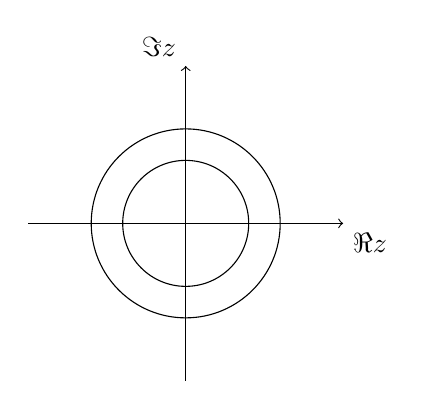
\begin{tikzpicture}[scale=1]
		\draw[->] (-2,0) -- (2,0) node[anchor=north west] {$\Re{z}$};
		\draw[->] (0,-2) -- (0,2) node[anchor=south east] {$\Im{z}$};
		\clip (-2,-2) rectangle (2,2);
		\draw (0,0) circle (1.2cm);
		\draw (0,0) circle (0.8cm);
		\end{tikzpicture}
	\end{center}
	Se per assurdo la serie converge in $z \implies$ per il teorema precedente  avremmo convergenza in ogni sfera con raggio minore di $\abs{\frac{1}{z}}$. e quindi anche in $w$ questo nega l'ipotesi.ASSURDO.
\end{proof}
\observation
Come è fatto l'insieme su cui si ha convergenza??\\
segue da queste due ultime proposizioni che se $\brackets{a_n:n\in\N}$ è una successione in $\C$ allora l'insieme $\brackets{z\in\C:\sum\limits_{n=0}^{+\infty}a_nz^n converge}$ è un cerchio.\\Sulla circonferenza non ci soffermaiamo a capire cosa accade poiché tutto può accadere.
\definition
Raggio di convergenza della serie $\sum\limits_{n=0}^{+\infty}a_nz^n\bydef \rho=\sup\brackets{r \geq 0 :\sum\limits_{n=0}^{+\infty}a_nz^n converge su B(0,r)}$
\observation
Il raggio di convergenza di una serie di potenze può essere $0$, un numero reale positivo o $+\infty$.
\observation
una definizione come $\rho=\inf\brackets{r \geq 0 :\sum\limits_{n=0}^{+\infty}a_nz^n non converge su B(0,r)}$ non sta in piedi poiché questo insieme potrebbe essere vuoto, mentre quello sopra non è mai vuoto, poerché $r=0$ c'è sempre poiché in $0$ si ha sempre convergenza. Ilsecondo potrebbe essere vuoto perché ci sono serie che convergono su tuttoil piano complesso e quindi non si avrebbe nessun $r$ fuori da quale non sia ha convergenza.\\
\proposition CRITERIO DELLA RADICE.\\
Data la serie di potenze $\sum\limits_{n=0}^{+\infty}a_nz^n$, sia $l=\lim\limits_{n\to+\infty}\sqrt[n]{\abs{a_n}}$.\\
Se questo limite esiste, allora il raggio di convergenza è
$\rho =
	\begin{cases}
		0				&	\text{se }l=+\infty\\
		\frac{1}{l} 	&	\text{se }l\in\left]0,+\infty\right[\\
		+\infty 		& 	\text{se }l=0
	\end{cases}
$
\proposition CRITERIO DEL RAPPORTO.\\
Data la serie di potenze $\sum\limits_{n=0}^{+\infty}a_nz^n$, sia $l=\lim\limits_{n\to+\infty}\frac{a_{n+1}}{a_n}$.\\
Se questo limite esiste, allora il raggio di convergenza è
$\rho =
\begin{cases}
0				&	\text{se }l=+\infty\\
\frac{1}{l} 	&	\text{se }l\in\left]0,+\infty\right[\\
+\infty 		& 	\text{se }l=0
\end{cases}
$
ESEMPIO::$e^z=\sum\limits_{n=0}^{+\infty}\frac{1}{n!}z^n$\\
$a_n=\frac{1}{n!} ...  \abs{\frac{a_{n+1}}{a_n}}=\frac{\frac{1}{(n+1)!}}{\frac{1}{n!}}=\frac{n!}{(n+1)!}=\frac{1}{n+1}\overset{n\to+\infty}{\to}0 \implies \rho=+\infty$\\
ESEMPIO::$sin(z)=\sum\limits_{n=0}^{+\infty}\frac{(-1)^nz^{2n+1}}{(2n+1)!}$ quindi
$a_n =
\begin{cases}
0		&	\text{se }n\text{ è pari}\\
...		&	\text{se }n\text{ è dispari}\\
\end{cases}
$\\
...\\
...\\
...\\
ESEMPIO::$sin(z)=\sum\limits_{n=0}^{+\infty}\frac{(-1)^nz^{2n}}{(2n)!}$ quindi
$a_n =
\begin{cases}
...		&	\text{se }n\text{ è pari}\\
0		&	\text{se }n\text{ è dispari}\\
\end{cases}
$\\
...\\
...\\
...\\
ESEMPIO:: $e^{iy}$ con $y\in \R$
\[e^{iy} = \sum\limits_{n=0}^{+\infty}\frac{1}{n!}(iy)^n = \sum\limits_{n=0}^{+\infty}\frac{1}{(2n)!}(iy)^{2n} + \sum\limits_{n=0}^{+\infty}\frac{1}{(2n+1)!}(iy)^{2n+1} = \]
\[ = \sum\limits_{n=0}^{+\infty}\frac{(-1)^n}{(2n)!}(y)^{2n} + i\sum\limits_{n=0}^{+\infty}\frac{(-1)^n}{(2n+1)!}(y)^{2n+1} = cos(y)+isin(y)\]
\begin{enumerate}
	\item $i^{2n}=\left(i^2\right)^n=(-1)^n$
	\item $i^{2n+1}=i\left(i^2\right)^n=i(-1)^n$
\end{enumerate}
ESEMPIO:: $e^{i\pi}+1=cos(\pi)+i\cdot sin(\pi)=0$\\
ESEMPIO:: $\sum\limits_{n=0}^{+\infty}z^n=\frac{1}{1-z}$ con $\rho=1$
ESEMPIO:: Sia $f(x)=\frac{1}{1+x^2}=\frac{1}{1-(-x^2)} = \sum\limits_{n=0}^{+\infty}(-x^2)^n=\sum\limits_{n=0}^{+\infty}(-1)^nx^{2n}$\\
QUI GRAFICO ..............\\
..........................\\
Questa serieconverge esclusivamente per $\abs{x}<1$, mentre la funzione $f$ è definita su tutto $ \R$, $f\in \cntclass{\infty}( \R; \R)$\\
In $\C$, lafunzione $f(z)=\frac{1}{1+z^2}$ è la somma della serie $\sum\limits_{n=0}^{+\infty}(-1)^nz^{2n}$ che ha raggio di convergenza  $\rho=1$. Infatti, $f(z)$ è singolare sia in $z=i$ sia in $z=-i$.\\
ALTRO GRAFICO::::::::::::::::\\
................................\\

\subsection{Serie di Taylor}
ESEMPIO:: $ln(1+z)$. Calcolare la Serie di Taylor.
\[D\left[ln(1+z)\right] = \frac{1}{1+z} = \sum\limits_{n=0}^{+\infty}(-1)^nz^n\]
\[\int \sum\limits_{n=0}^{+\infty}(-1)^nz^n dz = \sum\limits_{n=0}^{+\infty}\frac{(-1)^n}{n+1}z^{n+1}=\sum\limits_{n=1}^{+\infty}\frac{(-1)^{n-1}}{n}z^n\]
\begin{lemma}
	\label{lemma:taylor_rad_convergency}
	Sia $\brackets{a_n:n \in \N}$ una successione a valori in $\C$. Le serie:
	\[\sum_{n=0}^{+\infty} a_n z^n ,\qquad \sum_{n=1}^{+\infty} n a_n z^{n-1} \qquad\text{e}\qquad \sum_{n=0}^{+\infty} \frac{a_n}{n+1}z^{n+1}\]
	hanno lo stesso raggio di convergenza
	\begin{proof}
		Omessa
	\end{proof}
\end{lemma}

\definition
Sia $r\in \R$ con $r>0$. La funzione $f$ si dice analitica su $\left]-r,r\right[ \bydef f(x)=\sum\limits_{n=0}^{+\infty}a_nx^n \quad \forall x\in\left]-r,r\right[$ per opportuni $a_n\in \R$
\observation
In altre parole chiamiamo analitica una funzione che può essere scritta come somma di una serie di potenze convergente su $\left]-r,r\right[$ \\
ESEMPIO:: $x\to e^x$ è analitica su $ \R$\\
ESEMPIO:: $x\to\frac{1}{1+x^2}$ è analitica su $\left]-1,1\right[$\\
\proposition
Se $f$ è analitica su $\left]-r;r\right[$ per $r\in \R$ e $r>0 \implies f\in \cntclass{0}(\left]-r,r\right[; \R)$
\begin{proof}
	$f$ è analitica  allora posso scriverla come $f=\sum\limits_{n=0}^{+\infty}a_nx^n$ cioè la funzione è limite di una serie, se la serie converge totalmente allora converge uniformemente. Il limite uniforme di funzioni continue(in questo caso polinomi) è una funzione continua. cioè la $f$ è continua.
\end{proof}
\proposition PROP+PROOF\\
Sia $f:\left]-r,r\right[\to \R$ e $f$ analitica su $\left]-r,r\right[ \bydef f(x)=\sum\limits_{n=0}^{+\infty}a_nx^n \implies$ ho convergenza totale $\implies$ ho convergenza uniforme di funzioni continue
\[\implies f\in \cntclass{0}(\left]-r,r\right[; \R),\quad a_0=f(0)\]
La serie delle derivate $\sum\limits_{n=0}^{+\infty}na_nx^{n-1}$ converge totalmente su $\left]-r,r\right[$ cioè
\[\sum\limits_{n=0}^{+\infty}f'(x)=\sum\limits_{n=0}^{+\infty}na_nx^{n-1} \uconvarrow g\]
\[\sum\limits_{n=0}^{+\infty}fn(0)\to f(0), f_n\in ????????????\]
Allora la serie delle derivate converge alla derivata della serie
\[\implies \in \cntclass{1}(\left]-r,r\right[; \R),\quad a_1=f'(0)\]
Questo ragionmento può essere ripetuto:
\[\implies \forall k\in\N,\quad f\in \cntclass{k}(\left]-r,+r\right[),\quad a_k=k!f^{(k)}(0)\]
e analogamente
\[f\in \cntclass{\infty}(\left]-r,r\right[; \R),\quad f(x)=\sum\limits_{n=0}^{+\infty}\frac{1}{n!}f^{(n)}(0)x^n\]
\observation Qui abbiamo detto se $f$ è analitica $\implies \ldots$, vorrei fare un qualche tipo di viceversa per poter capire se $f$ è analitica o no.
\proposition
Sia $f:\left]-r,r\right[\to \R$
\begin{center}
	$\left.\begin{matrix}
	f\in \cntclass{\infty}(\left]-r,r\right[; \R)\\
	\sum\limits_{n=0}^{+\infty}\frac{1}{n!}f^{(n)}(0)x^n\text{ converge totalmente su } \left]-r,r\right[\\
	\end{matrix}\right\}\implies f$ è analitica  .....
\end{center}
Per avere $f$ analitica  necessariamente come ipotesi deve esserci $f\in \cntclass{\infty}$ e $f$ che si può scrivere come sviluppo in serie di Taylor,dalla proposizione precedente. Questo basta? NO\\
ESEMPIO:: $f(x)=\left\{\begin{matrix}0&& x=0\\e^{-\frac{1}{x^2}}&&x\ne 0\end{matrix}\right.$
\begin{center}
	\begin{tikzpicture}[scale=1]
	%\draw[->] (0,-4) -- (0,4) node[anchor=north west] {$x$};
	%\draw[->] (-0.1,0) -- (1.2,0) node[anchor=south east] {$y$};
	%\clip (-4,0) rectangle (4,1);
	%\draw[domain=-4:4,smooth,variable=\x] plot ({\x},{{-1/(\x*\x)}});
	\end{tikzpicture}
\end{center}
\begin{enumerate}
	\item $f\in \cntclass{\infty}( \R; \R)$
	\item $\sum\limits_{n=0}^{+\infty}\frac{1}{n!}f^{(n)}(0)x^n$ converge totalmente su $ \R$
	\item $f(x)\ne\sum\limits_{n=0}^{+\infty}\frac{1}{n!}f^{(n)}(0)x^n$
\end{enumerate}
\begin{enumerate}
	\item Vediamo se è $\cntclass{0}$, quindi calcolo $\lim\limits_{x\to 0^{+}}f(x)=\lim\limits_{x\to 0^{-}}f(x)=0=f(0)\implies f\in \cntclass{0}( \R; \R)$.\\
	Ora calcoliamo la derivata fuori dallo zero, ne facciamo il limite per $x\to 0$ da destra e da sinitra e vediamo cosa succede.\\
	Se $x\ne 0$, $f'(x)=\frac{2}{x^3}e^{-\frac{1}{x^3}}$ e $\lim\limits_{x\to 0^{+}}f'(x)=\lim\limits_{x\to 0^{-}} = 0 \implies f\in \cntclass{1}( \R; \R)$\\
	..........\\
	ancora una derivata.......\\
	..........\\
	Continuando a derivare  avremmo sempre un rapporto di polinomi che moltiplica un esponenziale, e l'esponenziale vince sempre. quindi fa $0$.
	itero il ragionamento......\\
	.......\\
	\item In (1) abbiamo visto  che tutte le derivate nello zero si annullavano, cioè
	\[\forall n\in\N, f^{(n)}(0)=0 \implies \sum\limits_{n=0}^{+\infty}\frac{1}{n!}f^{(n)}(0)x^n\]
	è la serie identicamente nulla  che banalmente converge totalmente su tutto $ \R$
	\item Anche osservandoil grafico è chiaro che la $f$ non è la funzione identicamente nulla cioè è diversa dal suo sviluppo in serie
	\[f(x)\ne\sum\limits_{n=0}^{+\infty}\frac{1}{n!}f^{(n)}(0)x^n\]
\end{enumerate}
Il Problema nasce dall'$o(x^n)$ che scriviamo alla fine dello sviluppo n-esimo di questa funzione, perché l'intorno in cui si ha $o(x^n)$ diventa sempre più piccolo.
GRAFICO...\\
GRAFICO...\\
Mandando l'ordine $n$ all'infinito, l'intervallo su cui si ha l'o piccolo tende a diventare un punto (lo zero). Quindi abbiamo l'ugualianza tra la funzione e il suo sviluppo solo nell'origine.????????NON COMPRESA????\\
????????NON COMPRESA????\\
????????NON COMPRESA????\\
????????NON COMPRESA????\\
Completiamo le ipotesi con la prossima proposizione:
\proposition
Sia $f:\left]-r,r\right[\to \R$
\begin{center}
	$\left.\begin{matrix}
	f\in \cntclass{\infty}(\left]-r,r\right[; \R)\\
	\exists H,K >0 :\forall n\in\N \sup\limits_{\left]-r,r\right[}\abs{f^{(n)}(x)} \leq HK^n\\
	\end{matrix}\right\}
	\implies f(x)=\sum\limits_{n=0}^{+\infty}\frac{1}{n!}f^{(n)}(0)x^n$
\end{center}
\observation
L'ipotesi centrale ............. qui non c'è
\observation
Sia $\sum\limits_{n=0}^{+\infty}(z,w)^n$ una serie di potenze in due variabili.\\
Quando abbiamo due variabili, non si può parlare di raggio di convergenza. Questa serie è una serie geometrica che converge sse $\abs{zw}<1$. è  difficile parlare di raggio di convergenza  perché essendo $z,w\in\C$, se per una variabile servono due dimensioni per due variabili servono quattro dimensioni , e anche se non riusciamo a fare il disegno è evidente che l'insieme su cui la serie converge non è un cerchio(sfera).
\begin{example}[Esempi di Sviluppi in serie di Taylor]
	\label{ex:tay_series_examples}
	\begin{description}
		\item $e^x=\sum\limits_{n=0}^{+\infty}\frac{1}{n!}x^n$
		\item $sin(x)=\sum\limits_{n=0}^{+\infty}\frac{(-1)^n}{(2n+1)!}x^{(2n+1)}$
		\item $sinh(x)=\sum\limits_{n=0}^{+\infty}\frac{1}{(2n+1)!}x^{(2n+1)}$
		\item $cos(x)=\sum\limits_{n=0}^{+\infty}\frac{(-1)^n}{(2n)!}x^{(2n)}$
		\item $cosh(x)=\sum\limits_{n=0}^{+\infty}\frac{1}{(2n)!}x^{(2n)}$
		\item $\frac{1}{1-x}=\sum\limits_{n=0}^{+\infty}x^n$
		\item $ln(1+x)=\sum\limits_{n=1}^{+\infty}\frac{(-1)^{n+1}}{n}x^n$
		\item $arctan(1+x)=\sum\limits_{n=0}^{+\infty}\frac{(-1)^{n}}{2n+1}x^{(2n+1)}$
		\item $\frac{1}{1+x^2}=\sum\limits_{n=0}^{+\infty}(-1)^nx^2n$
		\item $\sum\limits_{n=0}^{+\infty}\frac{1}{n^\lambda}=\left\{\begin{matrix}\text{converge sse } \lambda >1\\ \text{diverge sse } \lambda  \leq 1 \end{matrix}\right.$
		\item $\sum\limits_{n=0}^{+\infty}q^n=\left\{\begin{matrix}\text{converge sse } \abs{q}<1, S=\frac{1}{1-x}\\ \text{diverge sse } \abs{q}>1\text{ o }q=1\\\nexists \text{ sse } x=-1 \end{matrix}\right.$
	\end{description}
\end{example}
\begin{exercise}
	\label{ex:deriv_func_with_taylor}
	Determinare le derivate delle funzioni
	\begin{itemize}[noitemsep]
		\item $x \to \sin x$
		\item $x \to \cos x$
		\item $x \to e^x$
	\end{itemize}
	utilizzando \fullref{ex:tay_series_examples}, il \fullref{lemma:taylor_rad_convergency} ed il \fullref{coro:deriv_serie_e_serie_derivate}.
\end{exercise}

\subsection{Serie di Fourier}
\definition
Siano $A\subseteq \R$, $f:A\to \R$ e $T>0$, $f$ è $T$-periodica $\bydef \forall x\in A
\left\{\begin{matrix}
x+T\in A\\f(x+T)=f(x)
\end{matrix}\right. $\\


ESEMPIO:: $\lfloor x \rfloor = \text{ parte intera } = \max\brackets{k\in\mathbb{Z}:k \leq x}$
\[\lfloor \pi \rfloor=3, \quad \lfloor \sqrt{2} \rfloor = 1 \quad \lfloor -e \rfloor = -3 \]
\begin{center}
	\begin{tikzpicture}
		\draw[->] (-4,0) -- (4,0) node[anchor=north west] {$x$};
		\draw[->] (0,-4) -- (0,4) node[anchor=south east] {$y$};

		\foreach \num in {-3,...,3} {
			\draw[line width=0.25mm] (\num , \num) -- (\num+1 , \num);
			\draw[fill=black] (\num , \num) circle (0.1cm);
			\draw (\num+1, \num) circle (0.1cm);
		}
	\end{tikzpicture}
\end{center}
è $1$-periodica.
ESEMPIO:: $mant(x)=\text{ mantissa di x } = x- \lfloor x \rfloor$
\begin{center}
	\begin{tikzpicture}
	\draw[->] (-4,0) -- (4,0) node[anchor=north west] {$x$};
	\draw[->] (0,-4) -- (0,4) node[anchor=south east] {$y$};

	\foreach \num in {-3,...,3} {
		\draw[line width=0.25mm] (\num , 0) -- (\num+1 , 1);
		\draw[fill=black] (\num , 0) circle (0.1cm);
		\draw (\num+1, 1) circle (0.1cm);
	}
	\end{tikzpicture}
\end{center}
è $1$-periodica.
\observation
La funzione costante è $T$-periodica $\forall T>0$, ma non ha un periodo minimo, per questo motivo non la consideriamo.
\observation
Sia $f:A\to \R$ $T$-periodica. Allora possiamo definire $\overline{f}:\overline{A}\to \R$ che sia $2\pi$-periodica data da:
\[x\to f\left(\frac{T}{2\pi}x\right),\quad \overline{A}=\frac{2\pi}{T}A\]
\proposition
Siano $A\subseteq \R$, $f:A\to \R$ e $T>0$\\
$f$ è $T$-periodica $\implies \forall n\in\N$, $f$ è $nT$-periodica.
\proposition
Sia $f:\left[0,2\pi\right[\to \R \implies \exists ! \hat{f}: \R\to \R$ t.c.: $\left\{\begin{matrix} \hat{f} 2\pi-periodica\\\hat{f}_{\left|\left[0,2\pi\right]\right.}=f\end{matrix}\right.$
\begin{proof}
	$\forall x\in \R. \exists ! \hat{x}\in\left[0,2\pi\right[$ t.c.: $x=2\pi\cdot k+\hat{x}$ con $k\in\mathbb{Z}$ e $k=\left[??????\right]$
	\[\hat{f}(x)=f(\hat{x})\]
\end{proof}
cioè se noi estendiamo una funzione definita su $\left[0,2\pi\right[$ a tutto $ \R$ otteniamo una funzione unica e periodica.
\observation
Con i polinomi di Taylor ........\\
........\\
........\\
........\\
........\\
........\\
\definition
Dati $2n+1$ numeri reali $a_0,a_1,\dotsc,a_n,b_1,\dotsc,b_n$ si dice polinomio trigonometrico di coefficienti $a_0,a_1,\dotsc,a_n,b_1,\dotsc,b_n$ la funzione:
\[\begin{array}{rcl} p: \left[-\pi,\pi\right] & \to &  \R \\ x & \to & \frac{a_0}{2}+\sum\limits_{k=1}^{N}\left(a_ncos(nx)+b_nsin(nx)\right) \end{array}\]
\observation
Essendo un'approssimazione, si deve aggiungere l'errore. Come è fatto?. Per far uscire conti giusti e comodi andrebbe usata la distanza quadratica , ma questo prevede una lunga parte introduttiva, noi allora lo stimiamo con la distanza infinita.
\definition
Date due successioni di numeri reali $\brackets{a_n:n\in\N}$,$\brackets{b_n:n\in\N\setminus\brackets{0}}$, si defininisce serie trigonometrica di coefficienti  $\brackets{a_n:n\in\N}$,$\brackets{b_n:n\in\N\setminus\brackets{0}}$ la serie
\[\begin{array}{rcl} \mathfrak{F}: \left[-\pi,\pi\right] & \to &  \R \\ x & \to & \frac{a_0}{2}+\sum\limits_{k=1}^{+\infty}\left(a_ncos(nx)+b_nsin(nx)\right) \end{array}\]
LEMMA::\\
Se $h,k\in\N$ valgono le seguenti uguaglianze:
\begin{description}
	\item[$\ast$]
	$\int_{-\pi}^{\pi} cos(hx)cos(kx)=
	\left\{\begin{matrix}
	0 &&h\ne k\\\pi&&0\ne h=k\\2\pi&&0=h=k
	\end{matrix}\right.$
	\item[$\ast$] $\int_{-\pi}^{\pi}cos(hx)sin(kx)= 0 $
	\item[$\ast$]
	$\int_{-\pi}^{\pi}sin(hx)sin(kx)=
	\left\{\begin{matrix}
	0 &&h\ne k\text{ oppure }h=k=0\\ \pi&&0\ne h=k
	\end{matrix}\right.$
\end{description}
ESERCIZIO:: IL POLINOMIO DI FOURIER FORNISCE LA MIGLIORE APPROSSIMAZIONE NEL SENSO DELLA DISTANZA QUADRATICA.\\
Sia $f: \intervalclose{-\pi}{\pi} \to \R$, quale è la funzione a lei più vicina nel senso della distanza quadratica?\\
Fisso $N\in\N$ e prendo il polinomio trigonometrico di grado $N$
\[p_N(x)=\trigonpol{n}{1}{N}\]
con $a_0,a_1,\dotsc,a_n,b_1,\dotsc,b_n\in \R$, il problema è quello di minimizzare $d_2(f,p_n)$ quindi un problema di minimo. Stiamo cercando i coefficienti del polinomio trigonometrico quindi studiamo una funzione $\varphi(a_0,a_1,\dotsc,a_N,b_1,\dotsc,b_N) = \sqrt{\int_{-\pi}^{\pi}\left[f(x)-p_n(x)\right]^2}\integrald{x}$.\\
Essendo la funzione radice quadrata monotona crescente ne studiamo solo il radicando:
\[\varphi(a_0,a_1,\dotsc,a_N,b_1,\dotsc,b_N)=\int_{-\pi}^{\pi}\left[\trigonpol{n}{1}{N}-f(x)\right]^2dx\]
\observation
con $f\in \cntclass{1}$:
\[F(\alpha,\beta,x)=\int_{\alpha}^{\beta}f(x,t)\integrald{t}\]
\[\partial_\alpha F(\alpha,\beta,x)=-f(x,\alpha)\integrald{t}\]
\[\partial_\beta F(\alpha,\beta,x)=f(x,\beta)\integrald{t}\]
\[\nabla_x F(\alpha,\beta,x)=\int_{\alpha}^{\beta}\nabla_xf(x,t)\integrald{t}\]
Qudindi applicando al nostro caso otteniamo
\[\partial_{a_0}\varphi = \int_{-\pi}^{\pi}\partial_{a_0}\left(\left[\trigonpol{n}{1}{N}-f(x)\right]^2\right)\integrald{x}=\]
\[ = \int_{-\pi}^{\pi} \frac{1}{2}2\left(\trigonpol{n}{1}{N}-f(x)\right)\integrald{x}=\]
\[ =  \int_{-\pi}^{\pi} \frac{a_0}{2}\integrald{x} + \]
\[\int_{-\pi}^{\pi} a_1cos(x)\integrald{x} +
\ldots +
\int_{-\pi}^{\pi} a_Ncos(Nx)\integrald{x} + \]
\[\int_{-\pi}^{\pi} b_1sin(x)\integrald{x} +
\ldots +
\int_{-\pi}^{\pi} b_Nsin(Nx)\integrald{x} - \]
\[ \int_{-\pi}^{\pi} f(x)\integrald{x} = \]
L'integrale di una sinusoide su un multiplo intero del periodo è $0$ quindi
\[=\pi a_0-\int_{-\pi}^{\pi}f(x)\integrald{x}\]
Calcolando direttamente anche le derivate seconde si ottiene che
\[\partial^2_{a_0a_0}=\pi\quad\partial^2_{a_0a_n}=0\quad\partial^2_{a_0b_n}=0\quad\forall n=1,\dotsc,N\]

\[\partial_{a_k}\varphi = \int_{-\pi}^{\pi}\partial_{a_k}\left(\left[\trigonpol{n}{1}{N}-f(x)\right]^2\right)\integrald{x}=\]
\[ = \int_{-\pi}^{\pi} 2cos(kx) \left[\trigonpol{n}{1}{N}-f(x)\right]\integrald{x}=\]
\[ =  \cancel{\int_{-\pi}^{\pi} a_0cos(kx)\integrald{x}} + \]
\[\cancel{\int_{-\pi}^{\pi} 2a_1cos(x)cos(kx)\integrald{x}} +
\ldots +
\int_{-\pi}^{\pi} 2a_kcos(kx)cos(kx)\integrald{x}
\ldots +
\cancel{\int_{-\pi}^{\pi} 2a_Ncos(Nx)cos(kx)\integrald{x}} + \]
\[\cancel{\int_{-\pi}^{\pi} 2b_1sin(x)cos(kx)\integrald{x}} +
\ldots +
\cancel{\int_{-\pi}^{\pi} 2b_ksin(kx)cos(kx)}\integrald{x}
\ldots +
\cancel{\int_{-\pi}^{\pi} 2b_Nsin(Nx)cos(kx)\integrald{x}} - \]
\[\int_{-\pi}^{\pi} 2f(x)cos(kx)\integrald{x} = \]
E anche applicando il lemma
\[=2\pi\left[a_k-\int_{-\pi}^{\pi}f(x)cos(kx)\integrald{x}\right]\]
Calcolando direttamente anche le derivate seconde si ottiene che
\[\partial^2_{a_ka_0}=\pi\quad\partial^2_{a_ka_n}=
\left\{\begin{matrix}
0&&n\ne k\\2\pi&&n=k
\end{matrix}\right.
\quad\partial^2_{a_kb_n}=0\quad\forall n=1,\dotsc,N\]

\[\partial_{b_k}\varphi = \int_{-\pi}^{\pi}\partial_{b_k}\left(\left[\trigonpol{n}{1}{N}-f(x)\right]^2\right)\integrald{x}=\]
\[ = \int_{-\pi}^{\pi} 2sin(kx) \left[\trigonpol{n}{1}{N}-f(x)\right]\integrald{x}=\]
\[ =  \cancel{\int_{-\pi}^{\pi} a_0sin(kx)\integrald{x}} + \]
\[\cancel{\int_{-\pi}^{\pi} 2a_1cos(x)sin(kx)\integrald{x}} +
\ldots +
\cancel{\int_{-\pi}^{\pi} 2a_kcos(kx)sin(kx)}\integrald{x}
\ldots +
\cancel{\int_{-\pi}^{\pi} 2a_Ncos(Nx)sin(kx)\integrald{x}} + \]
\[\cancel{\int_{-\pi}^{\pi} 2b_1sin(x)sin(kx)\integrald{x}} +
\ldots +
\int_{-\pi}^{\pi} 2b_ksin(kx)sin(kx)\integrald{x}
\ldots +
\cancel{\int_{-\pi}^{\pi} 2b_Nsin(Nx)sin(kx)\integrald{x}} - \]
\[\int_{-\pi}^{\pi} 2f(x)sin(kx)\integrald{x} = \]
E anche applicando il lemma
\[=2\pi\left[b_k-\int_{-\pi}^{\pi}f(x)cos(kx)\integrald{x}\right]\]
Calcolando direttamente anche le derivate seconde si ottiene che
\[\partial^2_{b_ka_0}=\pi\quad\partial^2_{b_ka_n}=
\left\{\begin{matrix}
0&&n\ne k\\2\pi&&n=k
\end{matrix}\right.
\quad\partial^2_{b_kb_n}=0\quad\forall n=1,\dotsc,N\]
Si verifica la condizione $\nabla\varphi = 0$ con
\begin{description}
	\item[$\ast$] $a_0=\frac{1}{\pi}\int_{-\pi}^{\pi}f(x)\integrald{x}$
	\item[$\ast$] $a_k=\frac{1}{\pi}\int_{-\pi}^{\pi}f(x)cos(kx)\integrald{x}$
	\item[$\ast$] $b_k=\frac{1}{\pi}\int_{-\pi}^{\pi}f(x)sin(kx)\integrald{x}$
\end{description}
La matrice Hessiana di $\varphi$ risulta \[H_{\varphi}=\left[\begin{matrix}
\pi&&0&&0&&\ldots&&0\\
0&&2\pi&&0&&\ldots&&0\\
0&&0&&2\pi&&\ldots&&0\\
\vdots&&\vdots&&\vdots&&\ddots&&\vdots\\
0&&0&&0&&0\ldots&&2\pi
\end{matrix}\right]\]
è una matrice diagonale quindi si leggono direttamente tutti gli autovalori che sono strettamente positivi quindi la forma quadratica è definita positiva ed il punto in questione è un punto di minimo assoluto.
\definition
Sia $f: \intervalclose{-\pi}{\pi} \to \R$, i coefficienti di Fourier di $f$ sono (ovviamente $f$ deve essere tale da ammetterli finiti):
\[a_0=\frac{1}{\pi}\int_{-\pi}^{\pi}f(x)\integrald{x}\]
\[a_k=\frac{1}{\pi}\int_{-\pi}^{\pi}f(x)cos(kx)\integrald{x}\quad k\in\N\setminus{\brackets{0}}\]
\[b_k=\frac{1}{\pi}\int_{-\pi}^{\pi}f(x)sin(kx)\integrald{x}\quad k\in\N\setminus{\brackets{0}}\]
La serie di Fourier di $f$ è
\[\trigonpol{k}{1}{+\infty}\]
\proposition
Sia $F: \intervalclose{-\pi}{\pi} \to \R$ la somma della serie trigono metrica definita dai coefficienti $\brackets{a_n:n\in\N}$ e $\brackets{a_n:n\in\N\setminus\brackets{0}}$ e la serie trigonometrica converge uniformemente allora $F$ è una funzione continua e
\[a_k=\frac{1}{\pi}\int_{-\pi}^{\pi}F(x)cos(kx)\integrald{x}\quad k\in\N\]
\[b_k=\frac{1}{\pi}\int_{-\pi}^{\pi}F(x)sin(kx)\integrald{x}\quad k\in\N\setminus{\brackets{0}}\]
ESEMPIO+DIMOSTRAZIONE:::\\
sia $f(x)=\trigonpol{n}{1}{+\infty}$. Allora:\\
\[a_0=\frac{1}{\pi}\int_{-\pi}^{\pi}f(x)\integrald{x}=\frac{1}{\pi}\int_{-\pi}^{\pi}\trigonpol{n}{1}{+\infty}\integrald{x}=\]
\[
= \frac{1}{\pi}\int_{-\pi}^{\pi}\frac{a_0}{2} +
\frac{1}{\pi}\int_{-\pi}^{\pi}\left(\sum\limits_{n=1}^{+\infty} a_ncos(nx)\right)\integrald{x} +
\frac{1}{\pi}\int_{-\pi}^{\pi}\left(\sum\limits_{n=1}^{+\infty} b_ncos(nx)\right)\integrald{x}
\]
Poiché si ha convergenza uniforme si può portare l'integrale dentro la sommatoria.
\[
= \frac{1}{\pi}\int_{-\pi}^{\pi}\frac{a_0}{2} +
\cancel{\frac{1}{\pi}\sum\limits_{n=1}^{+\infty}\int_{-\pi}^{\pi} a_ncos(nx)\integrald{x}} +
\cancel{\frac{1}{\pi}\sum\limits_{n=1}^{+\infty}\int_{-\pi}^{\pi} b_ncos(nx)\integrald{x}}=
\]
\[=\frac{1}{\pi}\frac{a_0}{2}\left(\pi-(-\pi)\right)=a_0\]


\[a_k=\frac{1}{\pi}\int_{-\pi}^{\pi}f(x)cos(kx)\integrald{x}=\]
\[\frac{1}{\pi}\left[
\cancel{\int_{-\pi}^{\pi}\frac{a_0}{2}cos(kx)\integrald{x}}+
\int_{-\pi}^{\pi}\left(\sum\limits_{n=1}^{+\infty}a_ncos(nx)cos(kx)\right)\integrald{x}+
\cancel{\int_{-\pi}^{\pi}\left(\sum\limits_{n=1}^{+\infty}b_nsin(nx)cos(kx)\right)\integrald{x}}
\right]=\]
\[\frac{1}{\pi}\left[
\cancel{\int_{-\pi}^{\pi}\left(\sum\limits_{n=1}^{k-1} a_ncos(nx)cos(kx)\right)\integrald{x}}+
\int_{-\pi}^{\pi}a_kcos(kx)cos(kx)\integrald{x}+
\cancel{\int_{-\pi}^{\pi}\left(\sum\limits_{n=k+1}^{+\infty}a_ncos(nx)cos(kx)\right)}\integrald{x}
\right]=\]
\[=\frac{1}{\pi}\pi a_k=a_k\]

\[b_k=\frac{1}{\pi}\int_{-\pi}^{\pi}f(x)sin(kx)\integrald{x}=\]
\[\frac{1}{\pi}\left[
\cancel{\int_{-\pi}^{\pi}\frac{a_0}{2}sin(kx)\integrald{x}}+
\int_{-\pi}^{\pi}\left(\sum\limits_{n=1}^{+\infty}a_ncos(nx)sin(kx)\right)\integrald{x}+
\cancel{\int_{-\pi}^{\pi}\left(\sum\limits_{n=1}^{+\infty}b_nsin(nx)sin(kx)\right)\integrald{x}}
\right]=\]
\[\frac{1}{\pi}\left[
\cancel{\int_{-\pi}^{\pi}\left(\sum\limits_{n=1}^{k-1} a_ncos(nx)sin(kx)\right)\integrald{x}}+
\int_{-\pi}^{\pi}a_kcos(kx)sin(kx)\integrald{x}+
\cancel{\int_{-\pi}^{\pi}\left(\sum\limits_{n=k+1}^{+\infty}a_ncos(nx)sin(kx)\right)}\integrald{x}
\right]=\]
\[=\frac{1}{\pi}\pi b_k=b_k\]
\observation
Se $d_2(f,\text{polinomio di Fourier})$ \`{e} minima $\implies$ il polinomio di Fourier \`{e} costruito con i coefficienti di Fourier di $f$.
\observation
Se $f$ \`{e} somma di una serie di funzioni $\implies$ i coefficienti della serie sono i coefficienti di Fourier.
\observation
Funzioni diverse possono avere gli stessi coefficienti di Fourier, cio\`{e} $\exists f,g$ con $f\ne g$ ma $f$ e $g$  hanno gli stessi coefficienti di Fourier.
ESEMPIO::
\begin{center}
	\begin{tikzpicture}
		\draw[->] (-2,0) -- (2,0) node [anchor=north west]{$x$};
		\draw[->] (0,0) -- (0,2);
		\clip (-2,0) rectangle (2,2);
		\draw[domain=-2:2,smooth,red,variable=\x] plot ({\x},{1}) node{$f$};
		\draw[domain=-2:2,smooth,blue,variable=\x] plot ({\x},{1}) node{$g$};
	\end{tikzpicture}
	SISTEMARE,
\end{center}
\observation
I coefficienti di Fourier non possono identificare univocamente puntualmente una funzione.
\subsubsection{Punto Di Vista Geometrico}
In $R^2$ Ci sono $2$ vettori $\hat{i},\hat{j}$ della base, se $\underline{v}\in \R^2 \implies \underline{v}=v_1\cdot \hat{i}+v_2\cdot \hat{j}$ con $v_1,v_2$ componenti di $\underline{v}$\\
Calcolo delle componenti:
\[\underline{v}\cdot \hat{i} = v_1\cdot \hat{i\cdot }\hat{i}+v_2\cdot \hat{j}\cdot \hat{i}=v_1\]
\[\underline{v}\cdot \hat{j} = v_1\cdot \hat{i}\cdot \hat{j}+v_2\cdot \hat{j}\cdot \hat{j}=v_2\]
Questo vale perché $\hat{i},\hat{j}$ è una base ortonormale.
In $R^3$ Ci sono $3$ vettori $\hat{i},\hat{j},\hat{k}$ della base, se $\underline{v}\in \R^3 \implies \underline{v}=v_1\hat{i}+v_2\hat{j}+v_3\hat{k}$ con $v_1,v_2,v_3$ componenti di $\underline{v}$\\
Calcolo delle componenti:
\[ v_1=\underline{v}\cdot \hat{i}\quad v_2=\underline{v}\cdot \hat{j}\quad v_3=\underline{v}\cdot \hat{k}  \]
In $R^n$ Ci sono $n$ vettori $e_1,e_2,\dotsc,e_n$ della base, se $\underline{v}\in \R^n \implies \underline{v}=v_1\cdot e_1+v_2\cdot e_2+\ldots+v_n\cdot e_n=\sum\limits_{k=1}^{n}v_k\cdot e_k$ con $v_1,v_2,\dotsc,v_n$ componenti di $\underline{v}$\\
Calcolo delle componenti:
\[v_k=\underline{v}\cdot e_k\]
\\
Con le Serie di Fourier su esegue la stessa operazione sullo spazi $\cntclass{0}(\intervalclose{-\pi}{\pi}; \R)$. Come elementi di base si ha un insieme di funzioni:
\begin{enumerate}
	\item $c_0:x\to 1$
	\item $c_1:x\to cos(x)$
	\item $c_2:x\to cos(2x)$
	\item $\ldots$
	\item $c_n:x\to cos(nx)$
	\item $s_1:x\to sin(x)$
	\item $s_2:x\to sin(2x)$
	\item $\ldots$
	\item $s_n:x\to sin(nx)$
\end{enumerate}
Si possono osservare due cose:
\begin{enumerate}
	\item Sono tutte funzioni linearmente indipendenti, poiché l'unica combinazione lineare di questi elementi che da l'elemento nullo è quella a coefficenti tutti nulli.
\end{enumerate}
\definition
Il prodotto scalare in $\cntclass{0} \bydef \left<f,g\right>=\int_{-\pi}^{\pi}f(x)g(x)\integrald{x}$
Altre simbologie usate sono: $ f\bullet g $, $(f|g)$
\observation linearità
\[\left<(\alpha\cdot f+\beta\cdot g), h \right>= \int_{-\pi}^{pi} (\alpha\cdot f(x)+\beta\cdot g(x))\cdot h(x) \integrald{x}=\]
\[=\int_{-\pi}^{pi} \left[\alpha\cdot f(x)\cdot h(x)+\beta\cdot g(x)\cdot h(x) \right]\integrald{x}= \]
\[=\alpha\int_{-\pi}^{pi} \cdot f(x)\cdot h(x) \integrald{x}+\beta\int_{-\pi}^{pi} \cdot g(x)\cdot h(x) \integrald{x} =\]
\[\alpha\left<f,h\right>+\beta\left<g,h\right>\]

Ripetiamolo stesso ragionamento applicato in $ \R^2, \R^3,$ e $ \R^n$ per ricavare le componenti, possiamo fare questo perché abbiamo una base e abbiamo definito un prodotto scalare.\\
Se $f(x)=\trigonpol{n}{1}{+\infty} \implies $
\[a_0=\frac{1}{\pi}\int_{-\pi}^{\pi}f(x)dxs=\frac{1}{\pi}\left<f,c_0\right> \]
\[a_k=\frac{1}{\pi}\int_{-\pi}^{\pi}f(x)cos(kx)\integrald{x}=\frac{1}{\pi}\left<f,c_k\right> \]
\[b_k\frac{1}{\pi}\int_{-\pi}^{\pi}f(x)sin(kx)\integrald{x}=\frac{1}{\pi}\left<f,s_k\right>\]
Quindi come prima le componenti di un vettore si ottengono moltiplicando(prodotto scalare) il vettore per gli elementi della base.\\
PER IL LEMMA:\\
\[
\left<c_h,c_k\right>=
\left\{\begin{matrix}
0&&h\ne k\\
2\pi&&0=h=k\\
\pi&&0\ne h=k\\
\end{matrix}\right.
\]
\[ \left<c_h,s_k\right>=0\]
\[
\left<s_h,s_k\right>=
\left\{\begin{matrix}
0&&h\ne k\\
\pi&&0\ne h=k\\
\end{matrix}\right.
\]
Il prodotto scalare di elementi diversi è nullo quindi la base è ortogonale, ma non è ortonormale in quanto il prodotto scalare tra due elementi diversi della base non è unitario.(ecco perché gli $\frac{1}{\pi})$ e $\frac{a_0}{2}$)\\
In generale in geometria non è difficile normalizzare una base, è sufficiente dividere tutti gli elementi per la loro norma. In questo caso decidiamo di non applicare questo ragionamento poiché la norma vale $\sqrt{\pi}$ e se normalizziamo dobbiamo aggiungere questo termini ......\\
Il prodotto scalare in $\cntclass{0}$ è molto legato alla $d_2$ infatti:
\[\norm{f}_2=\sqrt{\left<f,f\right>}=\sqrt{\int_{-\pi}^{\pi}f(x)\cdot f(x)\integrald{x}}\sqrt{\int_{-\pi}^{\pi}\left[f(x)\right]^2dx}\]
Continuano le analogie:\\
In $ \R^2$ ........\\
In $ \R^3$ .........\\
.....\\
......\\
......\\
.....\\
Passando in dimensione infinita, abbiamo una funzione $f$ (come vettore $\underline{v}$) nello spazio, e fare il polinomio di Fourier  vuole dire proiettare la funzione $f$ in uno spazio fatto dai primi $2n+1$ elementi della base che è uno spazio di dimensione finita.\\
\\
Esempio:::: Non ogni funzione ammette coefficienti di Fourier finiti. La funzione
\[\begin{array}{rcl} f: \left[-\pi,\pi\right] & \to &  \R \\
x & \to & \left\{\begin{matrix} 0 && x=0\\\frac{1}{x^2}&&x\ne 0 \end{matrix}\right. \end{array}\]
non ammette coefficienti di Fourier finiti.\\
Esempio::: Una funzione può ammettere tutti i coefficienti di Fourier finiti ed una serie di Fourier convergente, ma ad un limite diverso da $f$.La funzione.
\[\begin{array}{rcl} f: \left[-\pi,\pi\right] & \to &  \R \\
x & \to & \left\{\begin{matrix} -1 && x<0\\1&&x>0 \end{matrix}\right. \end{array}\]
ha coefficienti di Fourier
\[a_k=0\quad\forall k,\quad\quad \left\{\begin{matrix}0 && k\text{ dispari }\\ \frac{4}{k\pi}&& k \text{ pari } \end{matrix}\right.\]
e serie di Fourier
\[ F_f(x)= \frac{4}{\pi}\sum\limits_{k=0}^{+\infty}\frac{sin(2h+1)x}{2h+1} \]
questa serie converge puntualmente in $0$ ma $F_f(0)\ne f(0)$\\

ESEMPIO:: Due funzioni diverse possono avere gli stessi coefficienti di Fourier:
\[\begin{array}{rcl} f: \left[-\pi,\pi\right] & \to &  \R \\
x & \to & \left\{\begin{matrix} -1 && x<0\\0&&x= 0\\1&&x>0 \end{matrix}\right.\end{array}\]
\[\begin{array}{rcl} g: \left[-\pi,\pi\right] & \to &  \R \\
x & \to & \left\{\begin{matrix} -1 && x<0\\\pi&&x= 0\\1&&x>0 \end{matrix}\right.\end{array}\]
\observation
Sia $f$ una funzione pari $\implies bn=0 \forall n=1,2,\dotsc,+\infty$
\observation
Sia $f$ una funzione dispari $\implies an=0 \forall n=0,1,,\dotsc,+\infty$
\observation
Siano
\[f(x)=\frac{a_0}{2}+\sum\limits_{n=}^{+\infty}\left(a_ncos(nx)+b_nsin(nx)\right)\]
\[\varphi(x)=\frac{\alpha_0}{2}+\sum\limits_{n=}^{+\infty}\left(\alpha_ncos(nx)+\beta_nsin(nx)\right)\]
Allora
\[ F(x)=(f+\varphi)(x)=\frac{A_0}{2}+\sum\limits_{n=}^{+\infty}\left(A_ncos(nx)+B_nsin(nx)\right)\]
con $A_n=a_n+\alpha_n$. $B_n=b_n+\beta_n$.
cioè i coefficienti di Fourier dipendono linearmente dalla funzione.\\
Esempio::: $B_3=\frac{1}{\pi}\int_{-\pi}^{\pi}F(x)sin(3x)\integrald{x}=\frac{1}{\pi}\int_{-\pi}^{\pi}(f(x)+\varphi(x))sin(3x)\integrald{x}=$\\
$\frac{1}{\pi}\left[\int_{-\pi}^{\pi}f(x)sin(3x)\integrald{x}+\int_{-\pi}^{\pi}\varphi(x)sin(3x)\integrald{x}\right]=b_3+\beta_3$\\
Sia $f(x)=\frac{a_0}{2}+\sum\liminf_{n=1}^{+\infty}\left(a_ncos(nx)+b_ncos(nx)\right)$ allora $F=4f=\frac{A_0}{2}+\sum\limits_{n=1}^{+\infty}\left(A_ncos(nx)+B_ncos(nx)\right)$ con $A_n=4a_n$, $B_n=4b_n$\\
ESEMPIO
Esempio:::$B_3=\frac{1}{\pi}\int_{-\pi}^{\pi}F(x)sin(3x)\integrald{x}=\frac{1}{\pi}\int_{-\pi}^{\pi}4f(x)sin(3x)\integrald{x}=4b_3$\\
\begin{definition}[Funzione Continua a Tratti]
	Siano $a,b\in \R$ con $a<b$, una funzione $f:\intervalclose{a}{b} \to \R$. Allora $f$ è \textbf{continua a tratti} se esiste un numero finito di punti $x_1,x_2,\dotsc,x_n$ tali che:
	\begin{enumerate}
		\item In ogni punto di $\intervalclose{a}{b}\setminus\brackets{x_1,x_2,\dotsc,x_n}$ f è continua
		\item $i=1,2,\dotsc,n$ esistono finiti entrambi i limiti:
		\[\lim\limits_{x\to x_i^{-}}f(x)\quad \lim\limits_{x\to x_i^{+}}f(x)\]
	\end{enumerate}
\end{definition}

\observation
Dato $A\subseteq \R$ e data una funzione $f:A \to \R$, se $x_0$ è punto interno ad $A$, è comoda la notazione
\[f(x-)=\lim\limits_{\xi\to x^{-}}f(\xi)\quad f(x+)=\lim\limits_{\xi\to x^{+}}f(\xi)\]
Ovviamente se $f$ è continua in $x$ allora $f(x-)=f(x)=f(x+)$
ESEMPIII:::\\
GRAFICO::::\\
GRAFICO::::\\
.......\\
.......\\
.......\\
.......\\
\proposition
Sia $f: \intervalclose{-\pi}{\pi} \to \R$, $f$ è continua a tratti $\implies$ esistono finiti tutti i coefficienti di Fourier di $f$
\proposition
Sia $f: \intervalclose{-\pi}{\pi} \to \R$,\\
-$f$ è continua a tratti\\
-$\forall \overline{x} \in\intervalclose{-\pi}{\pi}$, esistono finiti:\\
\[ \lim\limits_{x\to\overline{x}^{-}}=\frac{f(x)-f(\overline{x}-)}{x-\overline{x}} \]
\[ \lim\limits_{x\to\overline{x}^{+}}=\frac{f(x)-f(\overline{x}+)}{x-\overline{x}} \]
Allora:\\
La serie di Fourier di $f$ converge puntualmente in $\overline{x}$ e $F_f(\overline{x})=\frac{f(\overline{x}-)-\overline{x}+}{2}$ (che è il punto medio del salto.)
\observation NIENTE CUSPIDI E NIENTE TANGENZE VERTICALI.

\corollary
Sia $f: \intervalclose{-\pi}{\pi} \to \R$,\\
$f$ è continua a tratti.\\
Sia $\overline{x}\in\intervalclose{-\pi}{\pi}$ un punto in cui $f$ è derivabile. Allora la serie di Fourier $F_f$ di $f$ converge in $\overline{x}$ e $F_f(\overline{x})=f(\overline{x})$
\proposition
Sia $f: \intervalclose{-\pi}{\pi} \to \R$.Se:\\
\begin{description}
	\item[$\ast$] $f\in \cntclass{0}(\intervalclose{-\pi}{\pi}; \R)$
	\item[$\ast$] $\exists x_1,x_2,\dotsc,x_n\in\intervalclose{-\pi}{\pi}$ t.c.:
	\begin{description}
		\item[-] $f$ è derivabile in $x$
		\item[-] $f'$ continua in $x$
	\end{description}
	\item[$\ast$] $\forall i=1,2,\dotsc,n$ e $\forall x\in\intervalclose{-\pi}{\pi}$ esistono finiti
	\[\lim\limits_{x\to x_i^{-}}\frac{f(x)-f(x_i-)}{x-x_i}\qquad \lim\limits_{x\to x_i^{+}}\frac{f(x)-f(x_i+)}{x-x_i}\]

\end{description}
Allora\\
La serie di Fourier $F_f$ di $f$ converge a $f$ uniformemente su $\intervalclose{-\pi}{\pi}$
\corollary
Sia $f: \intervalclose{-\pi}{\pi} \to \R$, e $f\in \cntclass{1}(\intervalclose{-\pi}{\pi}; \R)$.\\
Allora la serie di Fourier di $F_f$ di $f$ converge uniformemente a $f$ su $\intervalclose{-\pi}{\pi}$.